\documentclass[10pt]{article}
%DIF LATEXDIFF DIFFERENCE FILE
%DIF DEL old_main.tex   Fri Apr  3 12:26:49 2020
%DIF ADD main.tex       Fri Apr  3 12:26:54 2020

% Manage page layout
\usepackage[margin=2.5cm, includefoot, footskip=30pt]{geometry}
\pagestyle{plain}
\setlength{\parindent}{0em}
\setlength{\parskip}{1em}
\renewcommand{\baselinestretch}{1}

%%%%%%%PACKAGES HERE%%%%%%%
\usepackage{tikz}
\usepackage{amsmath}
\usepackage{amssymb}
\usepackage{mathtools}
\usepackage{amsthm}
\usepackage{graphicx}
\usepackage{subcaption}
\usepackage{standalone}
\usepackage{booktabs}
\usepackage{setspace}
\usepackage[algoruled,lined]{algorithm2e}
\usepackage[noend]{algpseudocode}
\usepackage{wrapfig}
\usepackage{hyperref}
\usepackage{authblk}
\usepackage[toc,page]{appendix}
\usepackage{soul}
\usetikzlibrary{calc, shapes, patterns, decorations.pathreplacing}

\makeatletter
\def\BState{\State\hskip-\ALG@thistlm}
\makeatother

\newcommand{\R}{\mathbb{R}}
\newtheorem{theorem}{Theorem}
\usetikzlibrary{decorations.pathmorphing, decorations.pathreplacing, angles,
                quotes, calc, er, positioning}

\newtheorem{lemma}[theorem]{Lemma}
\def\arraystretch{1.5}

%DIF 41-42c41-42
%DIF < \title{Stability of defection, optimisation of strategies and the limits of
%DIF <        memory in the Prisoner's Dilemma.}
%DIF -------
\title{\textcolor{blue}{A theory of mind: Best responses to memory-one strategies. The limitations %DIF > 
of extortion and restricted memory.} \textcolor{red}{\st{Stability of defection, optimisation of strategies and the limits of
memory in the Prisoner's Dilemma COVER LETTER}}} %DIF > 
%DIF -------
\author[1, *]{Nikoleta E. Glynatsi}
\author[1]{Vincent A. Knight}

\affil[1]{Cardiff University, School of Mathematics, Cardiff, United Kingdom}
\affil[*]{Corresponding author: Nikoleta E. Glynatsi, glynatsine@cardiff.ac.uk}
\date{}
\setcounter{Maxaffil}{0}
\renewcommand\Affilfont{\itshape\small}
%DIF PREAMBLE EXTENSION ADDED BY LATEXDIFF
%DIF UNDERLINE PREAMBLE %DIF PREAMBLE
\RequirePackage[normalem]{ulem} %DIF PREAMBLE
\RequirePackage{color}\definecolor{RED}{rgb}{1,0,0}\definecolor{BLUE}{rgb}{0,0,1} %DIF PREAMBLE
\providecommand{\DIFaddtex}[1]{{\protect\color{blue}\uwave{#1}}} %DIF PREAMBLE
\providecommand{\DIFdeltex}[1]{{\protect\color{red}\sout{#1}}}                      %DIF PREAMBLE
%DIF SAFE PREAMBLE %DIF PREAMBLE
\providecommand{\DIFaddbegin}{} %DIF PREAMBLE
\providecommand{\DIFaddend}{} %DIF PREAMBLE
\providecommand{\DIFdelbegin}{} %DIF PREAMBLE
\providecommand{\DIFdelend}{} %DIF PREAMBLE
\providecommand{\DIFmodbegin}{} %DIF PREAMBLE
\providecommand{\DIFmodend}{} %DIF PREAMBLE
%DIF FLOATSAFE PREAMBLE %DIF PREAMBLE
\providecommand{\DIFaddFL}[1]{\DIFadd{#1}} %DIF PREAMBLE
\providecommand{\DIFdelFL}[1]{\DIFdel{#1}} %DIF PREAMBLE
\providecommand{\DIFaddbeginFL}{} %DIF PREAMBLE
\providecommand{\DIFaddendFL}{} %DIF PREAMBLE
\providecommand{\DIFdelbeginFL}{} %DIF PREAMBLE
\providecommand{\DIFdelendFL}{} %DIF PREAMBLE
%DIF HYPERREF PREAMBLE %DIF PREAMBLE
\providecommand{\DIFadd}[1]{\texorpdfstring{\DIFaddtex{#1}}{#1}} %DIF PREAMBLE
\providecommand{\DIFdel}[1]{\texorpdfstring{\DIFdeltex{#1}}{}} %DIF PREAMBLE
\newcommand{\DIFscaledelfig}{0.5}
%DIF HIGHLIGHTGRAPHICS PREAMBLE %DIF PREAMBLE
\RequirePackage{settobox} %DIF PREAMBLE
\RequirePackage{letltxmacro} %DIF PREAMBLE
\newsavebox{\DIFdelgraphicsbox} %DIF PREAMBLE
\newlength{\DIFdelgraphicswidth} %DIF PREAMBLE
\newlength{\DIFdelgraphicsheight} %DIF PREAMBLE
% store original definition of \includegraphics %DIF PREAMBLE
\LetLtxMacro{\DIFOincludegraphics}{\includegraphics} %DIF PREAMBLE
\newcommand{\DIFaddincludegraphics}[2][]{{\color{blue}\fbox{\DIFOincludegraphics[#1]{#2}}}} %DIF PREAMBLE
\newcommand{\DIFdelincludegraphics}[2][]{% %DIF PREAMBLE
\sbox{\DIFdelgraphicsbox}{\DIFOincludegraphics[#1]{#2}}% %DIF PREAMBLE
\settoboxwidth{\DIFdelgraphicswidth}{\DIFdelgraphicsbox} %DIF PREAMBLE
\settoboxtotalheight{\DIFdelgraphicsheight}{\DIFdelgraphicsbox} %DIF PREAMBLE
\scalebox{\DIFscaledelfig}{% %DIF PREAMBLE
\parbox[b]{\DIFdelgraphicswidth}{\usebox{\DIFdelgraphicsbox}\\[-\baselineskip] \rule{\DIFdelgraphicswidth}{0em}}\llap{\resizebox{\DIFdelgraphicswidth}{\DIFdelgraphicsheight}{% %DIF PREAMBLE
\setlength{\unitlength}{\DIFdelgraphicswidth}% %DIF PREAMBLE
\begin{picture}(1,1)% %DIF PREAMBLE
\thicklines\linethickness{2pt} %DIF PREAMBLE
{\color[rgb]{1,0,0}\put(0,0){\framebox(1,1){}}}% %DIF PREAMBLE
{\color[rgb]{1,0,0}\put(0,0){\line( 1,1){1}}}% %DIF PREAMBLE
{\color[rgb]{1,0,0}\put(0,1){\line(1,-1){1}}}% %DIF PREAMBLE
\end{picture}% %DIF PREAMBLE
}\hspace*{3pt}}} %DIF PREAMBLE
} %DIF PREAMBLE
\LetLtxMacro{\DIFOaddbegin}{\DIFaddbegin} %DIF PREAMBLE
\LetLtxMacro{\DIFOaddend}{\DIFaddend} %DIF PREAMBLE
\LetLtxMacro{\DIFOdelbegin}{\DIFdelbegin} %DIF PREAMBLE
\LetLtxMacro{\DIFOdelend}{\DIFdelend} %DIF PREAMBLE
\DeclareRobustCommand{\DIFaddbegin}{\DIFOaddbegin \let\includegraphics\DIFaddincludegraphics} %DIF PREAMBLE
\DeclareRobustCommand{\DIFaddend}{\DIFOaddend \let\includegraphics\DIFOincludegraphics} %DIF PREAMBLE
\DeclareRobustCommand{\DIFdelbegin}{\DIFOdelbegin \let\includegraphics\DIFdelincludegraphics} %DIF PREAMBLE
\DeclareRobustCommand{\DIFdelend}{\DIFOaddend \let\includegraphics\DIFOincludegraphics} %DIF PREAMBLE
\LetLtxMacro{\DIFOaddbeginFL}{\DIFaddbeginFL} %DIF PREAMBLE
\LetLtxMacro{\DIFOaddendFL}{\DIFaddendFL} %DIF PREAMBLE
\LetLtxMacro{\DIFOdelbeginFL}{\DIFdelbeginFL} %DIF PREAMBLE
\LetLtxMacro{\DIFOdelendFL}{\DIFdelendFL} %DIF PREAMBLE
\DeclareRobustCommand{\DIFaddbeginFL}{\DIFOaddbeginFL \let\includegraphics\DIFaddincludegraphics} %DIF PREAMBLE
\DeclareRobustCommand{\DIFaddendFL}{\DIFOaddendFL \let\includegraphics\DIFOincludegraphics} %DIF PREAMBLE
\DeclareRobustCommand{\DIFdelbeginFL}{\DIFOdelbeginFL \let\includegraphics\DIFdelincludegraphics} %DIF PREAMBLE
\DeclareRobustCommand{\DIFdelendFL}{\DIFOaddendFL \let\includegraphics\DIFOincludegraphics} %DIF PREAMBLE
%DIF LISTINGS PREAMBLE %DIF PREAMBLE
\RequirePackage{listings} %DIF PREAMBLE
\RequirePackage{color} %DIF PREAMBLE
\lstdefinelanguage{DIFcode}{ %DIF PREAMBLE
%DIF DIFCODE_UNDERLINE %DIF PREAMBLE
  moredelim=[il][\color{red}\sout]{\%DIF\ <\ }, %DIF PREAMBLE
  moredelim=[il][\color{blue}\uwave]{\%DIF\ >\ } %DIF PREAMBLE
} %DIF PREAMBLE
\lstdefinestyle{DIFverbatimstyle}{ %DIF PREAMBLE
	language=DIFcode, %DIF PREAMBLE
	basicstyle=\ttfamily, %DIF PREAMBLE
	columns=fullflexible, %DIF PREAMBLE
	keepspaces=true %DIF PREAMBLE
} %DIF PREAMBLE
\lstnewenvironment{DIFverbatim}{\lstset{style=DIFverbatimstyle}}{} %DIF PREAMBLE
\lstnewenvironment{DIFverbatim*}{\lstset{style=DIFverbatimstyle,showspaces=true}}{} %DIF PREAMBLE
%DIF END PREAMBLE EXTENSION ADDED BY LATEXDIFF

\begin{document}

\maketitle

\newpage

\begin{abstract}
    Memory-one strategies are a set of Iterated Prisoner's Dilemma strategies
    that have been praised for their mathematical tractability and performance
    against single opponents. This manuscript investigates \DIFaddbegin \DIFadd{a theory of mind: }\DIFaddend \textit{best
    response} memory-one strategies\DIFaddbegin \DIFadd{, }\DIFaddend as a multidimensional
    optimisation problem. \DIFdelbegin \DIFdel{Though extortionate memory-one strategies have gained
    much attention, we demonstrate that best response memory-one strategies do not behave in an extortionateway, and moreover, for memory one strategies to be
    evolutionary robust they need to be able to behave in a forgiving way}\DIFdelend \DIFaddbegin \DIFadd{We add to the literature that has shown that
    extortionate play is not always optimal by showing that optimal play is
    often not extortionate}\DIFaddend .
    We
    also provide evidence that memory-one strategies suffer from their limited
    memory in multi agent interactions and can be out performed by
    \DIFdelbegin \DIFdel{longer memory strategies}\DIFdelend \DIFaddbegin \DIFadd{optimised strategies with longer memory}\DIFaddend .
\end{abstract}

The Prisoner's Dilemma (PD) is a two player game used in understanding the
evolution of cooperative behaviour, formally introduced in~\cite{Flood1958}.
Each player has two options, to cooperate (C) or to defect (D). The decisions
are made simultaneously and independently. The normal form representation of the
game is given by:

\begin{equation}\label{equ:pd_definition}
    S_p =
    \begin{pmatrix}
        R & S  \\
        T & P
    \end{pmatrix}
    \quad
    S_q =
    \begin{pmatrix}
        R & T  \\
        S & P
    \end{pmatrix}
\end{equation}

where \(S_p\) represents the utilities of the row player and \(S_q\) the
utilities of the column player. The payoffs, \((R, P, S, T)\), are constrained
by \(T > R > P > S\) and \(2R > T + S\), and the most common values used in the
literature are \((R, P, S, T) = (3, 1, 0, 5)\)~\cite{Axelrod1981}.
The \DIFaddbegin \DIFadd{numerical experiments of our manuscript are carried out using these
payoff values.
The }\DIFaddend PD is a one shot game, however, it is commonly studied in a manner where the
history of the interactions matters. The repeated form of the game is called the
Iterated Prisoner's Dilemma (IPD).

Memory-one strategies are a set of IPD strategies that have been
studied thoroughly in the literature~\cite{Nowak1990, Nowak1993}, however, they have gained
most of their attention when a certain subset of memory-one strategies was
introduced in~\cite{Press2012}, the zero-determinant strategies (ZDs). In~\cite{Stewart2012} it
was stated that ``Press and Dyson have fundamentally changed the viewpoint on
the Prisoner's Dilemma''.
A special case of ZDs are extortionate strategies that choose their actions so that a linear relationship is forced
between the players' score ensuring that they will always
receive at least as much as their opponents. ZDs are
indeed mathematically unique and are proven to be robust in pairwise
interactions, however, their true effectiveness in tournaments and
evolutionary dynamics has been questioned~\cite{adami2013, Hilbe2013b,
Hilbe2013, Hilbe2015, Knight2018, Harper2015}.

In\DIFdelbegin \DIFdel{a similar fashion to}\DIFdelend ~\cite{Press2012} the \DIFaddbegin \DIFadd{authors stated that ``Only a player with a theory of
mind about his opponent can do better, in which case Iterated Prisoner's Dilemma
is an Ultimatum Game''. The }\DIFaddend purpose of this work is to \DIFdelbegin \DIFdel{consider
a given memory-one strategy; however, whilst~\mbox{%DIFAUXCMD
\cite{Press2012} }\hspace{0pt}%DIFAUXCMD
found a way for a
player to manipulate a given opponent, this work will consider a
multidimensional optimisation approach }\DIFdelend \DIFaddbegin \DIFadd{investigate the first
part of this sentence, more specifically, }\DIFaddend to identify the best response \DIFdelbegin \DIFdel{to a }\DIFdelend \DIFaddbegin \DIFadd{strategy
with a theory of mind of a }\DIFaddend given group of opponents. The outcomes of our work
reinforce known results, namely that memory-one strategies must be forgiving to
be evolutionarily stable~\cite{Stewart2013, Stewart2016} and that longer-memory
strategies have a certain form of advantage over short memory
strategies~\cite{Hilbe2017, Pan2015}.

In particular, this work presents a \DIFdelbegin \DIFdel{compact method of
identifying the best response }\DIFdelend \DIFaddbegin \DIFadd{closed form algebraic expression for the utility
of a }\DIFaddend memory-one strategy against a given set of opponents, \DIFdelbegin \DIFdel{and evaluates whether it}\DIFdelend \DIFaddbegin \DIFadd{a compact method of
identifying it's best response to that given set of opponents essentially: a theory
of mind. The aim is
to evaluate whether a best response memory-one strategy }\DIFaddend behaves in a
zero-determinant way which in turn indicates whether it can be extortionate. \DIFdelbegin \DIFdel{This is also done in evolutionary settings}\DIFdelend \DIFaddbegin \DIFadd{We
do this using a linear algebraic approach presented in~\mbox{%DIFAUXCMD
\cite{Knight2019}}\hspace{0pt}%DIFAUXCMD
.
This is done in tournaments with and without self interactions}\DIFaddend . Moreover, we
introduce a \DIFdelbegin \DIFdel{well designed }\DIFdelend framework that allows the comparison of an optimal
\DIFdelbegin \DIFdel{memory one strategy and a more complex }\DIFdelend \DIFaddbegin \DIFadd{memory-one strategy and an optimised }\DIFaddend strategy which has a larger memory.
\DIFdelbegin \DIFdel{This
is used to identify conditions for which defection is stable; thus identifying
environments where cooperation will not occur. }\DIFdelend 

\DIFaddbegin \DIFadd{To illustrate the analytical results obtained in this manuscript a number of
numerical experiments are run. The source code for these experiments has been
written in a sustainable manner~\mbox{%DIFAUXCMD
\cite{Benureau2018}}\hspace{0pt}%DIFAUXCMD
.
It is open source (}\url{https://github.com/Nikoleta-v3/Memory-size-in-the-prisoners-dilemma}\DIFadd{)
and tested which ensures the validity of the results. It has also been archived
and can be found at~\mbox{%DIFAUXCMD
\cite{nikoleta_glynatsi_2019}}\hspace{0pt}%DIFAUXCMD
.
}

\DIFaddend \section{Methods\DIFdelbegin \DIFdel{and Results}\DIFdelend }
\DIFdelbegin \subsection{\DIFdel{Utility}}
%DIFAUXCMD
\addtocounter{subsection}{-1}%DIFAUXCMD
\DIFdelend 

One specific advantage of memory-one strategies is their mathematical
tractability. They can be represented completely as an element of \(\R^{4}_{[0, 1]}\). This
originates from~\cite{Nowak1989} where it is stated that if a strategy is
concerned with only the outcome of a single turn then there are four possible
`states' the strategy could be in; both players cooperated (\(CC\)),
the first player cooperated whilst the second player defected (\(CD\)),
the first player defected whilst the second player cooperated (\(DC\)) and
both players defected (\(DD\)).
Therefore, a memory-one strategy can be denoted by the probability vector of
cooperating after each of these states; \(p=(p_1, p_2, p_3, p_4) \in \R_{[0,1]}
^ 4\).

In~\cite{Nowak1989} it was shown that it is not necessary to simulate the play
of a strategy $p$ against a memory-one opponent $q$. Rather this exact behaviour
can be modeled as a stochastic process, and more specifically as a Markov chain
whose corresponding transition matrix \(M\) is
given by Eq.~\ref{eq:transition_matrix}. The long run steady state probability
vector \(v\), which is the solution to \(v M = v\), can be
combined with the payoff matrices of Eq.~\ref{equ:pd_definition} to give the expected
payoffs for each player. More specifically, the utility for a memory-one
strategy \(p\) against an opponent \(q\), denoted as \(u_q(p)\), is given by
Eq.~\ref{eq:press_dyson_utility}.

\begin{equation}\label{eq:transition_matrix}
    \resizebox{.5\hsize}{!}{$M = \left[\begin{matrix}p_{1} q_{1} & p_{1} \left(- q_{1} + 1\right) & q_{1} \left(- p_{1} + 1\right) & \left(- p_{1} + 1\right) \left(- q_{1} + 1\right)\\p_{2} q_{3} & p_{2} \left(- q_{3} + 1\right) & q_{3} \left(- p_{2} + 1\right) & \left(- p_{2} + 1\right) \left(- q_{3} + 1\right)\\p_{3} q_{2} & p_{3} \left(- q_{2} + 1\right) & q_{2} \left(- p_{3} + 1\right) & \left(- p_{3} + 1\right) \left(- q_{2} + 1\right)\\p_{4} q_{4} & p_{4} \left(- q_{4} + 1\right) & q_{4} \left(- p_{4} + 1\right) & \left(- p_{4} + 1\right) \left(- q_{4} + 1\right)\end{matrix}\right]$}
\end{equation}


\begin{equation}\label{eq:press_dyson_utility}
    u_q(p) = v \cdot (R, S, T, P).
\end{equation}

This manuscript has explored the form of \(u_q(p)\), to the authors knowledge no
previous work has done this, and \DIFdelbegin \DIFdel{it proves }\DIFdelend \DIFaddbegin \DIFadd{Theorem~\ref{theorem_one} states }\DIFaddend that \(u_q(p)\) is given by a ratio
of two quadratic forms~\cite{kepner2011}\DIFdelbegin \DIFdel{,
(Theorem~\ref{theorem_one})}\DIFdelend \DIFaddbegin \DIFadd{.
}

\begin{theorem}\label{theorem_one}
    \DIFadd{The expected utility of a memory-one strategy \(p\in\mathbb{R}_{[0,1]}^4\)
    against a memory-one opponent \(q\in\mathbb{R}_{[0,1]}^4\), denoted
    as \(u_q(p)\), can be written as a ratio of two quadratic forms}\DIFaddend :

    \begin{equation}\label{eq:optimisation_quadratic}
    u_q(p) = \frac{\frac{1}{2}pQp^T + cp + a}{\frac{1}{2}p\bar{Q}p^T + \bar{c}p + \bar{a}},
    \end{equation}
    \DIFdelbegin %DIFDELCMD < 

%DIFDELCMD < %%%
\DIFdel{where \(Q=Q(q), \bar{Q}=\bar{Q}(q)\) }\DIFdelend \DIFaddbegin \DIFadd{where \(Q, \bar{Q}\) }\DIFaddend \(\in \R^{4\times4}\) \DIFdelbegin \DIFdel{, \(c=c(q) \text{ and } \bar{c}=\bar{c}(q)\)
}\DIFdelend \DIFaddbegin \DIFadd{are square matrices defined by the
    transition probabilities of the opponent \(q_1, q_2, q_3, q_4\) as follows:
}

    \begin{center}
    \begin{equation}
    \resizebox{0.9\linewidth}{!}{\arraycolsep=2.5pt%
    \boldmath\(
    Q = \left[\begin{matrix}0 & 5 q_{4} \left(q_{1} - q_{3}\right) & - q_{4} \left(q_{1} - q_{2}\right) & \left(q_{1} - q_{4}\right) \left(q_{2} - 5 q_{3} - 1\right)\\5 q_{4} \left(q_{1} - q_{3}\right) & 0 & - 3 q_{4} \left(q_{2} - q_{3}\right) & \left(q_{3} - q_{4}\right) \left(5 q_{1} - 3 q_{2} - 2\right)\\- q_{4} \left(q_{1} - q_{2}\right) & - 3 q_{4} \left(q_{2} - q_{3}\right) & 0 & - \left(q_{2} - q_{4}\right) \left(q_{1} - 3 q_{3} - 1\right)\\\left(q_{1} - q_{4}\right) \left(q_{2} - 5 q_{3} - 1\right) & \left(q_{3} - q_{4}\right) \left(5 q_{1} - 3 q_{2} - 2\right) & - \left(q_{2} - q_{4}\right) \left(q_{1} - 3 q_{3} - 1\right) & 0\end{matrix}\right]\)},
    \end{equation}
    \begin{equation}\label{eq:q_bar_matrix}
    \resizebox{0.8\linewidth}{!}{\arraycolsep=2.5pt%
    \boldmath\(
    \bar{Q} =  \left[\begin{matrix}0 & - \left(q_{1} - q_{3}\right) \left(q_{2} - q_{4} - 1\right) & \left(q_{1} - q_{2}\right) \left(q_{3} - q_{4}\right) & \left(q_{1} - q_{4}\right) \left(q_{2} - q_{3} - 1\right)\\- \left(q_{1} - q_{3}\right) \left(q_{2} - q_{4} - 1\right) & 0 & \left(q_{2} - q_{3}\right) \left(q_{1} - q_{4} - 1\right) & \left(q_{1} - q_{2}\right) \left(q_{3} - q_{4}\right)\\\left(q_{1} - q_{2}\right) \left(q_{3} - q_{4}\right) & \left(q_{2} - q_{3}\right) \left(q_{1} - q_{4} - 1\right) & 0 & - \left(q_{2} - q_{4}\right) \left(q_{1} - q_{3} - 1\right)\\\left(q_{1} - q_{4}\right) \left(q_{2} - q_{3} - 1\right) & \left(q_{1} - q_{2}\right) \left(q_{3} - q_{4}\right) & - \left(q_{2} - q_{4}\right) \left(q_{1} - q_{3} - 1\right) & 0\end{matrix}\right]\)}.
    \end{equation}
    \end{center}

    \DIFadd{\(c \text{ and } \bar{c}\) }\DIFaddend \(\in \R^{4 \times 1}\) \DIFdelbegin \DIFdel{, \(a=a(q) \text{ and } \bar{a}=\bar{a}(q) \in \R.\)
}\DIFdelend \DIFaddbegin \DIFadd{are similarly defined by:
}\DIFaddend 

    \DIFdelbegin \DIFdel{This }\DIFdelend \DIFaddbegin \begin{equation}\label{eq:q_matrix_numerator}
    \resizebox{0.6\linewidth}{!}{\arraycolsep=2.5pt%
    \boldmath\(c = \left[\begin{matrix}- 5 q_{1} q_{4}\\5 q_{4} \left(q_{3} - 1\right)\\q_{4} \left(2 q_{2} + 1\right)\\5 q_{1} q_{4} - 2 q_{2} q_{4} - q_{2} - 5 q_{3} q_{4} + 5 q_{3} - 3 q_{4} + 1\end{matrix}\right]\),}
    \end{equation}
    \begin{equation}\label{eq:q_matrix_denominator}
    \resizebox{0.3\linewidth}{!}{\arraycolsep=2.5pt%
    \boldmath\(\bar{c} = \left[\begin{matrix}q_{1} \left(q_{2} - q_{4} - 1\right)\\- \left(q_{3} - 1\right) \left(q_{2} - q_{4} - 1\right)\\- q_{1} q_{2} + q_{2} q_{3} + q_{2} - q_{3} + q_{4}\\q_{1} q_{4} - q_{2} - q_{3} q_{4} + q_{3} - q_{4} + 1\end{matrix}\right]\),
    }
    \end{equation}
    \DIFadd{and the constant terms \(a, \bar{a}\) are defined as \(a = 5 q_{4}\) and
    \(\bar{a} = - q_{2} + q_{4} + 1\).
}\end{theorem}

\DIFadd{The proof of Theorem~\ref{theorem_one} is given in
Appendix~\ref{appendix:theorem_one}.
Theorem~\ref{theorem_one} }\DIFaddend can be extended to consider multiple
opponents. The IPD is commonly studied in tournaments and/or Moran Processes
where a strategy interacts with a number of opponents. The payoff of a player in
such interactions is given by the average payoff the player received against
each opponent. More specifically the expected utility of a memory-one strategy
against \DIFdelbegin \DIFdel{a }\DIFdelend \(N\) \DIFdelbegin \DIFdel{number of }\DIFdelend opponents is given by:

\begin{align}\label{eq:tournament_utility}
       & \frac{1}{N} \sum\limits_{i=1} ^ {N} {u_q}^{(i)} (p) =
       \frac{\frac{1}{N} \sum\limits_{i=1} ^ {N} (\frac{1}{2} pQ^{(i)} p^T + c^{(i)} p + a^ {(i)})
       \prod\limits_{\tiny\begin{array}{l} j=1 \\ j \neq i \end{array}} ^
       N (\frac{1}{2} p\bar{Q}^{(j)} p^T + \bar{c}^{(j)} p + \bar{a}^ {(j)})}{\prod\limits_{i=1} ^ N (\frac{1}{2} p\bar{Q}^{(i)} p^T + \bar{c}^{(i)} p + \bar{a}^ {(i)})}.
\end{align}

\DIFaddbegin \DIFadd{Eq.~(\ref{eq:tournament_utility}) is the average score (using Eq.~(\ref{eq:optimisation_quadratic})) against the set of opponents.
}

\DIFaddend Estimating the utility of a memory-one strategy against any number of opponents
without simulating the interactions is the main result used in the rest of this manuscript.
It will be used to obtain best response memory-one strategies \DIFdelbegin \DIFdel{, in tournaments
and evolutionary dynamics, and }\DIFdelend \DIFaddbegin \DIFadd{in tournaments
with and without self interactions in order }\DIFaddend to explore the \DIFdelbegin \DIFdel{conditions under which defection
dominates cooperation.
}%DIFDELCMD < 

%DIFDELCMD < %%%
\subsection{\DIFdel{Stability of defection}}%DIFAUXCMD
\addtocounter{subsection}{-1}%DIFAUXCMD
%DIFDELCMD < \label{subsection:stability_defection}
%DIFDELCMD < 

%DIFDELCMD < %%%
\DIFdel{An immediate result from our formulation can be
obtained by evaluating the sign of Eq. \ref{eq:tournament_utility}'s derivative
at \(p=(0, 0, 0, 0)\). If at that point the
derivative is negative, then the utility of a player only decreases if they were
to change their behaviour, and thus }\textbf{\DIFdel{defection at that point is stable}}%DIFAUXCMD
\DIFdelend \DIFaddbegin \DIFadd{limitations of extortion
and restricted memory}\DIFaddend .

\DIFdelbegin %DIFDELCMD < \begin{lemma}\label{lemma:stability_of_defection}
%DIFDELCMD <     %%%
\DIFdel{In a tournament of \(N\) players \(\{q^{(1)}, q^{(2)}, \dots, q^{(N)} \}\)
    for \(q^{(i)} \in \R_{[0, 1]} ^ 4\)
    defection is stable if the transition probabilities of the
    opponents satisfy conditions Eq. \ref{eq:defection_condition_one} and Eq. \ref{eq:defection_condition_two}.
}\DIFdelend \DIFaddbegin \section{\DIFadd{Results}}\label{section:results}
\DIFaddend 

\DIFdelbegin %DIFDELCMD < \begin{equation}\label{eq:defection_condition_one}
%DIFDELCMD <         \sum_{i=1} ^ N (c^{(i)T} \bar{a}^{(i)} - \bar{c}^{(i)T} a^{(i)}) \leq 0
%DIFDELCMD <     \end{equation}
%DIFDELCMD < 

%DIFDELCMD <     %%%
\DIFdel{while,
}%DIFDELCMD < 

%DIFDELCMD <     \begin{equation}\label{eq:defection_condition_two}
%DIFDELCMD <         \sum_{i=1} ^ N \bar{a}^{(i)} \neq 0
%DIFDELCMD <     \end{equation}
%DIFDELCMD < \end{lemma}
%DIFDELCMD < 

%DIFDELCMD < \begin{proof}
%DIFDELCMD <     %%%
\DIFdel{For defection to be stable the derivative of the utility
    at the point \(p = (0, 0, 0, 0)\) must be negative.
}%DIFDELCMD < 

%DIFDELCMD <     %%%
\DIFdel{Substituting \(p = (0, 0, 0, 0)\) in
    Eq. \ref{eq:mo_tournament_derivative} gives:
}%DIFDELCMD < 

%DIFDELCMD <     \begin{equation}
%DIFDELCMD <         \left.\frac{d\sum\limits_{i=1} ^ {N} {u_q}^{(i)} (p)}{dp} \right\rvert_{p=(0,0,0,0)} =
%DIFDELCMD <     \sum_{i=1} ^ N \frac{(c^{(i)T} \bar{a}^{(i)} - \bar{c}^{(i)T} a^{(i)})}{(\bar{a}^{(i)})^2}
%DIFDELCMD <     \end{equation}
%DIFDELCMD < 

%DIFDELCMD <     %%%
\DIFdel{The sign of the numerator \( \displaystyle\sum_{i=1} ^ N (c^{(i)T} \bar{a}^{(i)} - \bar{c}^{(i)T} a^{(i)})\)
    can vary based on the transition probabilities of the opponents.
    The denominator can not be negative, and otherwise is always positive.
    Thus the sign of the derivative is negative if and only if
    \( \displaystyle\sum_{i=1} ^ N (c^{(i)T} \bar{a}^{(i)} - \bar{c}^{(i)T} a^{(i)}) \leq 0\).
}%DIFDELCMD < \end{proof}
%DIFDELCMD < 

%DIFDELCMD < %%%
\DIFdel{Consider a population for which defection is known to be stable. In that
population all the members will over time adopt the same behaviour; thus in such
population cooperation will never take over. This is demonstrated in
Fig.~\ref{fig:stability_of_defection}.
These have been simulated using~\mbox{%DIFAUXCMD
\cite{axelrodproject} }\hspace{0pt}%DIFAUXCMD
an open
source research framework for the study of the IPD.
}%DIFDELCMD < 

%DIFDELCMD < \begin{figure}[!htbp]
%DIFDELCMD <     \centering
%DIFDELCMD <     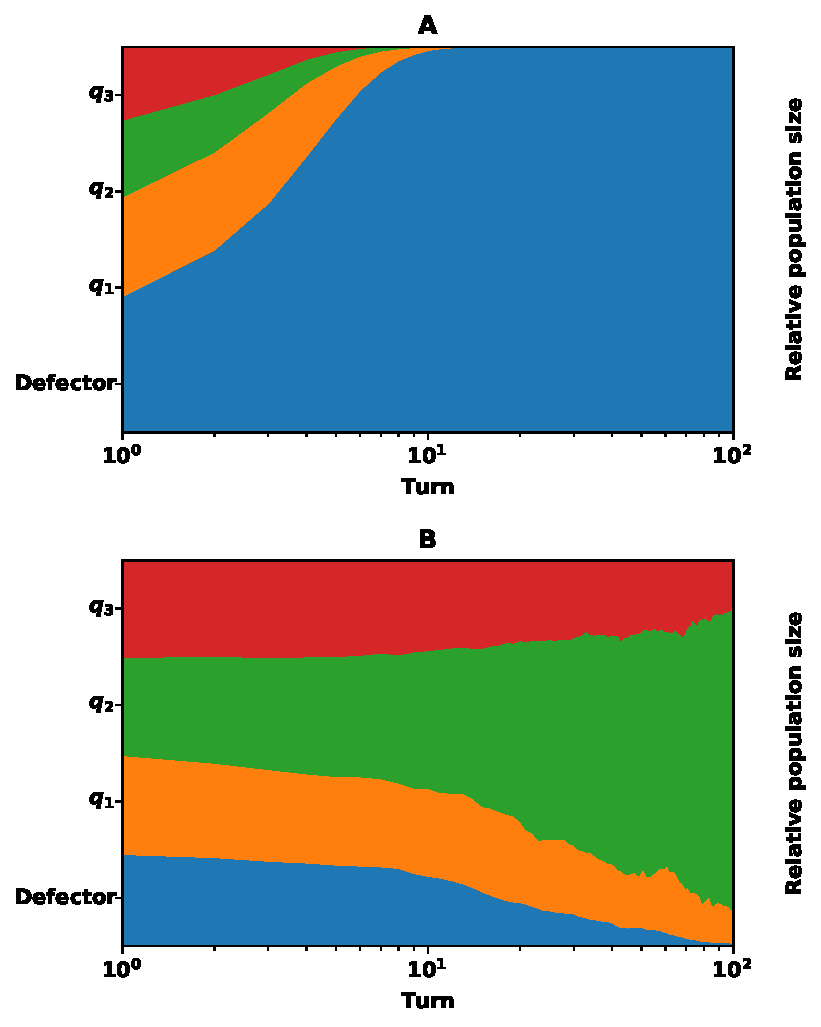
\includegraphics[width=.4\linewidth]{img/stability_of_defection_plots.pdf}
%DIFDELCMD <     %%%
%DIFDELCMD < \caption{%
{%DIFAUXCMD
\DIFdelFL{A. For \(q_{1}=(0.22199, 0.87073, 0.20672, 0.91861)\),
    $q_{2}=(0.48841, 0.61174, 0.76591, 0.51842)$ and
    $q_{3}=(0.2968, 0.18772, 0.08074, 0.73844)$, Eq.~\ref{eq:defection_condition_one} and
    Eq.~\ref{eq:defection_condition_two} hold and Defector takes over the
    population. B. For $q_{1}=(0.96703, 0.54723, 0.97268, 0.71482)$,
    $q_{2}=(0.69773, 0.21609, 0.97627, 0.0062)$ and
    $q_{3}=(0.25298, 0.43479, 0.77938, 0.19769)$, Eq.~\ref{eq:defection_condition_one} fails
    and Defector does not take over the population.}}%DIFAUXCMD
%DIFDELCMD < \label{fig:stability_of_defection}
%DIFDELCMD < \end{figure}
%DIFDELCMD < 

%DIFDELCMD < %%%
\subsection{\DIFdel{Best response memory-one strategies}}%DIFAUXCMD
\addtocounter{subsection}{-1}%DIFAUXCMD
%DIFDELCMD < \label{section:best_response_memory_one}
%DIFDELCMD < 

%DIFDELCMD < %%%
\DIFdel{As discussed ZDs have been acclaimed for their robustness
against a single opponent. ZDs are evidence that extortion works
in pairwise interactions, their behaviour ensures that the strategies will never
lose a game. However, this paper argues that in multi opponent interactions,
where the payoffs matter, strategies trying to exploit their opponents will
suffer.
Compared to ZDs, best response memory-one strategies, which have a
theory of mind of their opponents, utilise their behaviour in order to gain the
most from their interactions. The question that arises then is whether best
response strategies are optimal because they behave in an extortionate way.
}%DIFDELCMD < 

%DIFDELCMD < %%%
\DIFdel{To answer this question, we initially }\DIFdelend \DIFaddbegin \DIFadd{Here we }\DIFaddend define \textit{memory-one best response}
strategies as a multi dimensional optimisation problem given by:

\begin{equation}\label{eq:mo_tournament_optimisation}
    \begin{aligned}
    \max_p: & \ \sum_{i=1} ^ {N} {u_q}^{(i)} (p)
    \\
    \text{such that}: & \ p \in \R_{[0, 1]}
    \end{aligned}
\end{equation}

Optimising this particular ratio of quadratic forms is not trivial. It can be
verified empirically for the case of a single opponent that there exists at
least one point for which the definition of concavity does not hold.
The non concavity of \(u(p)\) indicates multiple local
optimal points. This is also intuitive. The best response against a cooperator,
\(q=(1, 1, 1, 1)\), is a defector \(p^*=(0, 0, 0, 0)\). The strategies
\(p=(\frac{1}{2}, 0, 0, 0)\) and \(p=(\frac{1}{2}, 0, 0, \frac{1}{2})\) are also
best responses. The approach taken here is to introduce a compact way of
constructing the discrete candidate set of all local optimal points, and evaluating
the objective function Eq.~\ref{eq:tournament_utility}. This gives the best
response memory-one strategy. The approach is given in
Theorem~\ref{memone_group_best_response}.

\DIFaddbegin \begin{theorem}\label{memone_group_best_response}

    \DIFadd{The optimal behaviour of a memory-one strategy player \(p^* \in \R_{[0, 1]} ^
    4\) against a set of \(N\) opponents \(\{q^{(1)}, q^{(2)}, \dots, q^{(N)} \}\)
    for \(q^{(i)} \in \R_{[0, 1]} ^ 4\) is given by:
    }

    \[p^* = \textnormal{argmax}\sum\limits_{i=1} ^ N  u_q(p), \ p \in S_q.\]

    \DIFadd{The set \(S_q\) is defined as all the possible combinations of:
    }

    {\scriptsize
    \begin{equation}\label{eq:s_q_set}
        S_q =
        \left\{p \in \mathbb{R} ^ 4 \left|
            \begin{aligned}
                \bullet\quad p_j \in \{0, 1\} & \quad \text{and} \quad \frac{d}{dp_k}
                \sum\limits_{i=1} ^ N  u_q^{(i)}(p) = 0 \\
                & \quad \text{for all} \quad j \in J \quad \&  \quad k \in K  \quad \text{for all} \quad J, K \\
                & \quad \text{where} \quad J \cap K = \O \quad
                \text{and} \quad J \cup K = \{1, 2, 3, 4\}.\\
                \bullet\quad  p \in \{0, 1\} ^ 4
            \end{aligned}\right.
        \right\}.
    \end{equation}
    }

    \DIFadd{Note that there is no immediate way to find the zeros of \(\frac{d}{dp}
    \sum\limits_{i=1} ^ N  u_q(p)\) where,
    }

    {\scriptsize
    \begin{align}\label{eq:mo_tournament_derivative}
        \frac{d}{dp} \sum\limits_{i=1} ^ {N} {u_q}^{(i)} (p) & = \displaystyle\sum\limits_{i=1} ^ {N}
        \frac{\left(pQ^{(i)} + c^{(i)}\right) \left(\frac{1}{2} p\bar{Q}^{(i)} p^T + \bar{c}^{(i)} p + \bar{a}^ {(i)}\right)}{\left(\frac{1}{2} p\bar{Q}^{(i)} p^T + \bar{c}^{(i)} p + \bar{a}^ {(i)}\right)^ 2}
        - \frac{\left(p\bar{Q}^{(i)} + \bar{c}^{(i)}\right) \left(\frac{1}{2} pQ^{(i)} p^T + c^{(i)} p + a^ {(i)}\right)}{\left(\frac{1}{2} p\bar{Q}^{(i)} p^T + \bar{c}^{(i)} p + \bar{a}^ {(i)}\right)^ 2}
    \end{align}
    }

    \DIFadd{For \(\frac{d}{dp} \sum\limits_{i=1} ^ N  u_q(p)\) to equal zero then:
    }

    {\scriptsize
    \begin{align}\label{eq:polynomials_roots}
        \displaystyle\sum\limits_{i=1} ^ {N}
        \left(pQ^{(i)} + c^{(i)}\right) \left(\frac{1}{2} p\bar{Q}^{(i)} p^T + \bar{c}^{(i)} p + \bar{a}^ {(i)}\right)
        - \left(p\bar{Q}^{(i)} + \bar{c}^{(i)}\right) \left(\frac{1}{2} pQ^{(i)} p^T + c^{(i)} p + a^ {(i)}\right)
        & = 0, \quad {while} \\
        \displaystyle\sum\limits_{i=1} ^ {N} \frac{1}{2} p\bar{Q}^{(i)} p^T + \bar{c}^{(i)} p + \bar{a}^ {(i)} & \neq 0.
    \end{align}}

\end{theorem}

\DIFadd{The proof of Theorem~\ref{memone_group_best_response} is given in
Appendix~\ref{appendix:memone_group_best_response}.
}\DIFaddend Finding best response memory-one strategies is analytically feasible using the
formulation of Theorem~\ref{memone_group_best_response} and resultant
theory~\cite{Jonsson2005}. However, for large systems building the resultant
becomes intractable. As a result, best responses will be estimated
heuristically using a numerical method, suitable for problems with local optima,
called Bayesian optimisation~\cite{Mokus1978}.

\DIFdelbegin \DIFdel{This is extended to evolutionary settings
. In these settings
}\DIFdelend \DIFaddbegin \DIFadd{In several evolutionary settings
such as Moran Processes }\DIFaddend self interactions are key. \DIFdelbegin \DIFdel{Self interactions can be incorporated in the
formulation that has been used so far. More specifically, the optimisation
problem of }\DIFdelend \DIFaddbegin \DIFadd{Previous work has
identified interesting results such as the appearance of self recognition
mechanisms when training strategies using evolutionary algorithms in Moran
processes~\mbox{%DIFAUXCMD
\cite{Knight2018}}\hspace{0pt}%DIFAUXCMD
. This aspect of reinforcement learning can be done for
best response memory-one strategies by incorporating the strategy itself in the
objective function as shown in }\DIFaddend Eq.~\ref{eq:mo_tournament_optimisation}\DIFdelbegin \DIFdel{is extended to include self interactions :
}\DIFdelend \DIFaddbegin \DIFadd{.
\(K\) is the number of self interactions that will take place.
}\DIFaddend 

\DIFdelbegin %DIFDELCMD < \begin{equation}\label{eq:mo_evolutionary_optimisation}
%DIFDELCMD < \begin{aligned}
%DIFDELCMD < \max_p: & \ \frac{1}{N} \sum\limits_{i=1} ^ {N} {u_q}^{(i)} (p) + u_p(p)
%DIFDELCMD < \\
%DIFDELCMD < \text{such that}: & \ p \in \R_{[0, 1]}
%DIFDELCMD < \end{aligned}
%DIFDELCMD < \end{equation}%%%
\DIFdelend \DIFaddbegin \begin{equation}\label{eq:mo_evolutionary_optimisation}
\begin{aligned}
\max_p: & \ \frac{1}{N} \sum\limits_{i=1} ^ {N} {u_q}^{(i)} (p) + \textcolor{blue}{K}u_p(p)
\\
\text{such that}: & \ p \in \R_{[0, 1]}
\end{aligned}
\end{equation}\DIFaddend 

For determining the memory-one best response \DIFdelbegin \DIFdel{in an evolutionary setting}\DIFdelend \DIFaddbegin \DIFadd{with self interactions}\DIFaddend , an
algorithmic approach is considered, called \textit{best response dynamics}. The
best response dynamics approach used in this manuscript is given by
Algorithm~\ref{algo:best_response_dynamics}.

\begin{center}
\begin{minipage}{.55\textwidth}
\begin{algorithm}[H]
       $p^{(t)}\leftarrow (1, 1, 1, 1)$\;
       \DIFdelbegin %DIFDELCMD < \While{$p^{(t)} \neq p ^{(t -1)}$}{
%DIFDELCMD <        $p^{(t + 1)} =  \text{argmax} \frac{1}{N} \sum\limits_{i=1} ^ {N} {u_q}^{(i)}
%DIFDELCMD <        (p^{(t + 1)}) + u_p^{(t)}(p^{(t + 1)})$\;
%DIFDELCMD <        }
%DIFDELCMD <        %%%
\DIFdelend \DIFaddbegin \While{$p^{(t)} \neq p ^{(t -1)}$}{
       $p^{(t + 1)} =  \text{argmax} \frac{1}{N} \sum\limits_{i=1} ^ {N} {u_q}^{(i)}
       (p^{(t)}) + \textcolor{blue}{K}u_{p^{(t)}}(p^{(t)})$\;
       }
       \DIFaddend \caption{Best response dynamics Algorithm}
       \label{algo:best_response_dynamics}
\end{algorithm}
\end{minipage}
\end{center}

\DIFaddbegin \DIFadd{Using this approach it would be possible to create a memory-one best response
strategy that updates on every generation of a Moran process to recalculate the
optimal behaviour given the population. This extension of the ``theory of mind''
is an interesting avenue for future work.
}

\DIFadd{In multi opponent settings,
where the payoffs matter, strategies trying to exploit their opponents will
suffer.
Compared to ZDs, best response memory-one strategies, which have a
theory of mind of their opponents, utilise their behaviour in order to gain the
most from their interactions. The question that arises then is whether best
response strategies are optimal because they behave in an extortionate way.
}

\DIFaddend The results of this section use Bayesian optimisation to generate a data set of best response
memory-one strategies \DIFdelbegin \DIFdel{, in tournaments and evolutionary dynamics whilst }\DIFdelend \DIFaddbegin \DIFadd{for }\DIFaddend \(N=2\) \DIFaddbegin \DIFadd{opponents}\DIFaddend .
The data set is available at~\cite{glynatsi2019}. It contains a total of 1000 trials
corresponding to 1000 different instances of a best response strategy in
tournaments \DIFdelbegin \DIFdel{and evolutionary dynamics}\DIFdelend \DIFaddbegin \DIFadd{with and without self interactions}\DIFaddend . For each trial a set of 2 opponents is
randomly generated and the memory-one best \DIFdelbegin \DIFdel{responses }\DIFdelend \DIFaddbegin \DIFadd{response }\DIFaddend against them is found.
\DIFdelbegin %DIFDELCMD < 

%DIFDELCMD < %%%
\DIFdel{The source code for the experiments presented in this manuscript has been written in a sustainable manner~\mbox{%DIFAUXCMD
\cite{Benureau2018}}\hspace{0pt}%DIFAUXCMD
.
It is open source (}%DIFDELCMD < \url{https://github.com/Nikoleta-v3/Memory-size-in-the-prisoners-dilemma}%%%
\DIFdel{)
and tested which ensures the validity of the results. It has also been archived
and can be found at~\mbox{%DIFAUXCMD
\cite{nikoleta_glynatsi_2019}}\hspace{0pt}%DIFAUXCMD
.
}%DIFDELCMD < 

%DIFDELCMD < %%%
\DIFdelend In order to investigate whether best responses
behave in an extortionate matter the SSE method \DIFaddbegin \DIFadd{described in }\DIFaddend ~\cite{Knight2019} is used. \DIFdelbegin \DIFdel{In~\mbox{%DIFAUXCMD
\cite{Knight2019} }\hspace{0pt}%DIFAUXCMD
it is proven that all extortionate ZDs reside on a triangular plane. For a given }\DIFdelend \DIFaddbegin \DIFadd{More
specifically,
in~\mbox{%DIFAUXCMD
\cite{Knight2019} }\hspace{0pt}%DIFAUXCMD
the point \(x^*\), in the space of memory-one strategies,
that is
the nearest extortionate strategy to a given strategy }\DIFaddend \(p\) \DIFdelbegin \DIFdel{, a strategy
\(x^*\) is defined as the nearest ZDs. The distance between
the two strategies is explicitly calculated and }\DIFdelend \DIFaddbegin \DIFadd{is
given by,
}

\begin{equation}\label{eqn:x_star_formula}
    x^* = {\left(C^{T}C\right)}^{-1}C^{T}\bar{p}
\end{equation}

\DIFadd{where \(\bar{p}=(p_1 - 1, p_2 - 1, p_3, p_4)\) and
}

\begin{equation}\label{eq:definition_of_C}
    C =
    \begin{bmatrix}
        R - P & R- P \\
        S - P & T- P \\
        T - P & S- P \\
        0     & 0 \\
    \end{bmatrix}.
\end{equation}

\DIFadd{Once this closest ZDs is found, the squared norm of the remaining error is }\DIFaddend referred to as \DIFdelbegin \DIFdel{the }\DIFdelend sum of squared errors
of prediction (SSE)\DIFdelbegin \DIFdel{; which corresponds to how far \(p\) }\DIFdelend \DIFaddbegin \DIFadd{:
}

\begin{equation}\label{eqn:x_SSError_formula}
    \text{SSE} = {\bar{p}} ^ T \bar{p} -
           \bar{p} C \left(C ^ T C \right) ^ {-1} C ^ T \bar{p}
         = {\bar{p}} ^ T \bar{p} - \bar{p} C x ^ *
\end{equation}

\DIFadd{Thus, SSE is defined as how far a strategy }\DIFaddend is from behaving as a \DIFdelbegin \DIFdel{ZDs. Thus, a }\DIFdelend \DIFaddbegin \DIFadd{ZD. A
}\DIFaddend high SSE implies \DIFdelbegin \DIFdel{non ZD, which in turn implies }\DIFdelend a non extortionate behaviour.
The \DIFdelbegin \DIFdel{SSE method has been applied to the data set.
A statistics summary
of the SSE distribution }\DIFdelend \DIFaddbegin \DIFadd{distributions of SSE }\DIFaddend for the best response in tournaments
\DIFdelbegin \DIFdel{and evolutionary dynamics }\DIFdelend \DIFaddbegin \DIFadd{(\(N=2\)) with and without self interactions (with \(K=1\)) are given in
Figure~\ref{fig:sse_distributions}. Moreover, a statistical summary of the SSE
distributions }\DIFaddend is given in Table~\ref{table:sserror_stats}.

\DIFaddbegin \begin{table}[!htbp]
    \begin{center}
    \resizebox{.8\columnwidth}{!}{%
    \begin{tabular}{lrrrrrrrrrrr}
        \toprule
        & mean & std  & 5\% & 50\% &  95\% & max & median & skew & kurt\\
        \midrule
    \textbf{Tournament without self interactions} & 0.34  & 0.40  & 0.028  & 0.17  &
    1.05  & 2.47  & 0.17  & 1.87 & 3.60 \\
    \textbf{Tournament with self interactions} & 0.17 & 0.23 & 0.01 &
    0.12 & 0.67 & 1.53 & 0.12 & 3.42 & 1.92 \\
        \bottomrule
    \end{tabular}}
    \end{center}
    \caption{\DIFaddFL{SSE of best response memory-one when \(N=2\)}}\label{table:sserror_stats}
\end{table}

\begin{figure}[!htbp]
    \begin{subfigure}{0.47\textwidth}
        \begin{center}
            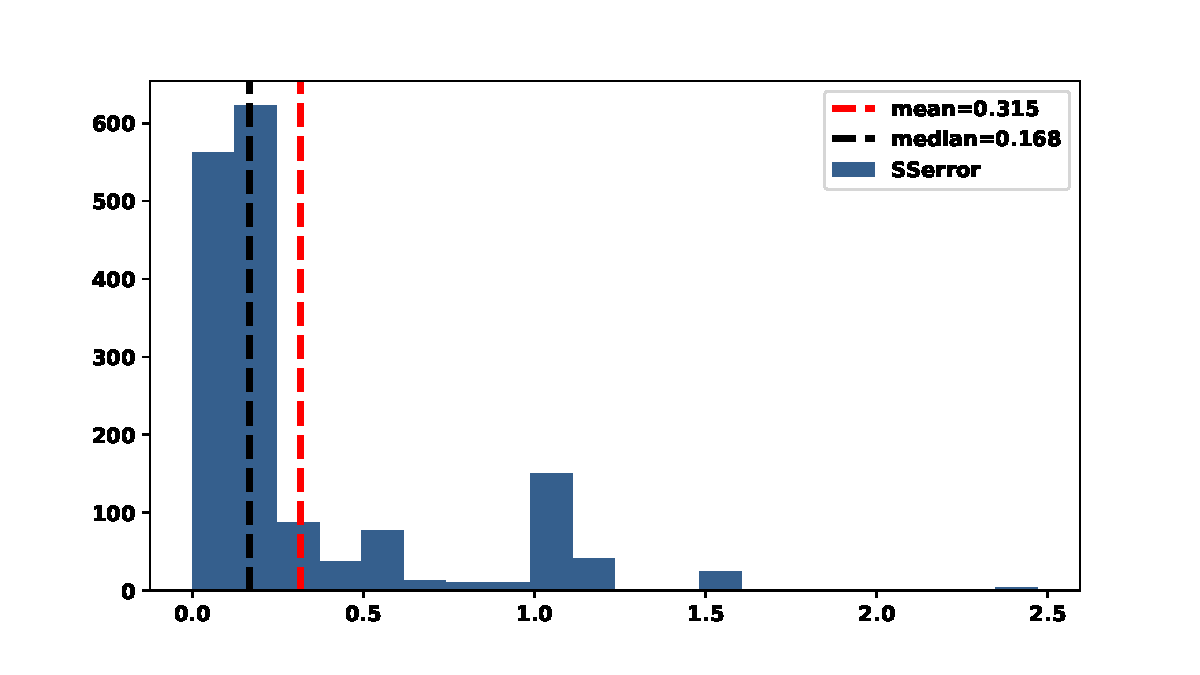
\includegraphics[width=\linewidth]{img/best_respones_sserror.pdf}
        \end{center}
        \caption{\DIFaddFL{SEE distribution for best response in tournaments without self interactions.}}
    \end{subfigure}\hfill
    \begin{subfigure}{0.47\textwidth}
        \begin{center}
            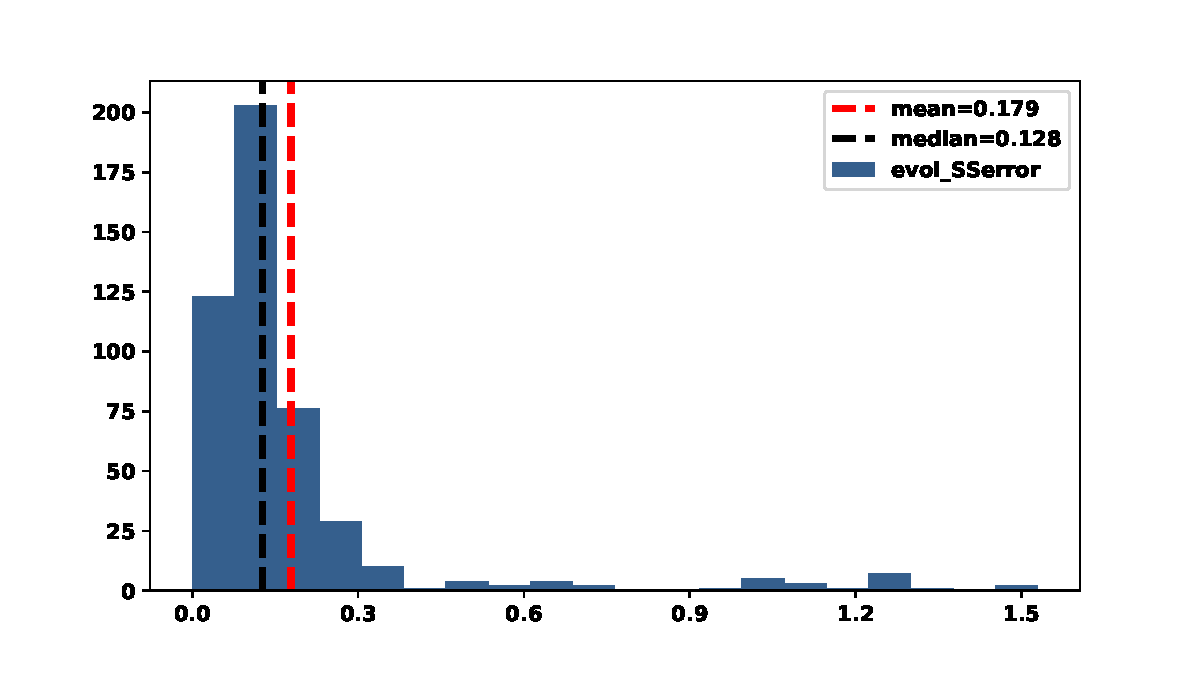
\includegraphics[width=\linewidth]{img/evo_sserror.pdf}
        \end{center}
        \caption{\DIFaddFL{SEE distribution for best response in tournaments with self interactions.}}
    \end{subfigure}
    \caption{\DIFaddFL{SEE distributions for best response in tournaments without and with self interactions.}}\label{fig:sse_distributions}
\end{figure}

\DIFaddend For the best response in tournaments \DIFaddbegin \DIFadd{that do not include self interactions }\DIFaddend the
distribution of SSE is skewed to the left, indicating that the best response
does exhibit ZDs behaviour and so could be extortionate, however, the best
response is not uniformly a ZDs. A positive measure of skewness and kurtosis\DIFdelbegin \DIFdel{indicates a }\DIFdelend \DIFaddbegin \DIFadd{,
and a mean of 0.34 indicate a }\DIFaddend heavy tail to the right. Therefore, in several
cases the strategy is not trying to extort its opponents.
\DIFdelbegin \DIFdel{Similarly the evolutionary best response strategy does not behave uniformly extortionately. A
larger value of both the
kurtosis and the skewness of the SSE distribution indicates that in evolutionary settings a }\DIFdelend \DIFaddbegin \DIFadd{In~\mbox{%DIFAUXCMD
\cite{Hilbe2018} }\hspace{0pt}%DIFAUXCMD
a similar behaviour is refereed to as the }\textit{\DIFadd{partner
strategy}}\DIFadd{. The partner
strategy aims to share the payoff for mutual cooperation, but it is ready
to fight back when being exploited. The partner strategy was designed, but the
best responses which are defined by their opponents seem to exhibit the same
behaviour.
}

\DIFadd{Similarly, when considering self interactions, the distribution of SSE for the best
response strategy has skewness and kurtosis that indicate a heavy tail to the
right. This indicates that evolutionary stable }\DIFaddend memory-one \DIFdelbegin \DIFdel{best response is even more adaptable .
}\DIFdelend \DIFaddbegin \DIFadd{strategies need to
more adaptable than a ZDs, and aim for mutual cooperation as well as
exploitation which is in line with the results of \mbox{%DIFAUXCMD
\cite{Hilbe2018} }\hspace{0pt}%DIFAUXCMD
where their
strategy was designed to adapt and was shown to be evolutionary stable. The
findings of this work show that an optimal strategy acts in the same way.
}\DIFaddend 

The difference between best responses in tournaments \DIFdelbegin \DIFdel{and in evolutionary
settings }\DIFdelend \DIFaddbegin \DIFadd{without and with self interactions
}\DIFaddend is further explored by Fig.~\ref{fig:behaviour_violin_plots}.
Though, no statistically significant differences have been found, from
Fig.~\ref{fig:behaviour_violin_plots}, it seems that \DIFdelbegin \DIFdel{evolutionary best
response }\DIFdelend \DIFaddbegin \DIFadd{the best
response that incorporate self interactions }\DIFaddend has a higher median $p_2$; which corresponds to the probability of cooperating
after receiving a defection. Thus, they are more likely to forgive after
being tricked. This is due to the fact that they could be playing against
themselves, and they need to be able to forgive so that future cooperation can
occur.

\DIFdelbegin %DIFDELCMD < \begin{table}
%DIFDELCMD < \begin{center}
%DIFDELCMD < \resizebox{.6\columnwidth}{!}{%
%DIFDELCMD < \begin{tabular}{lrrrrrrrrrrr}
%DIFDELCMD <     \toprule
%DIFDELCMD <     & mean & std  & 5\% & 50\% &  95\% & max & median & skew & kurt\\
%DIFDELCMD <     \midrule
%DIFDELCMD < \textbf{Tournament} & 0.34  & 0.40  & 0.028  & 0.17  &
%DIFDELCMD < 1.05  & 2.47  & 0.17  & 1.87 & 3.60 \\
%DIFDELCMD < \textbf{Evolutionary Setting} & 0.17 & 0.23 & 0.01 &
%DIFDELCMD < 0.12 & 0.67 & 1.53 & 0.12 & 3.42 & 1.92 \\
%DIFDELCMD <     \bottomrule
%DIFDELCMD < \end{tabular}}
%DIFDELCMD < \end{center}
%DIFDELCMD < %%%
%DIFDELCMD < \caption{%
{%DIFAUXCMD
\DIFdelFL{SSE of best response memory-one when \(N=2\)}}%DIFAUXCMD
%DIFDELCMD < \label{table:sserror_stats}
%DIFDELCMD < \end{table}
%DIFDELCMD < 

%DIFDELCMD < %%%
\DIFdelend \begin{figure}[!htbp]
    \centering
    \DIFdelbeginFL %DIFDELCMD < 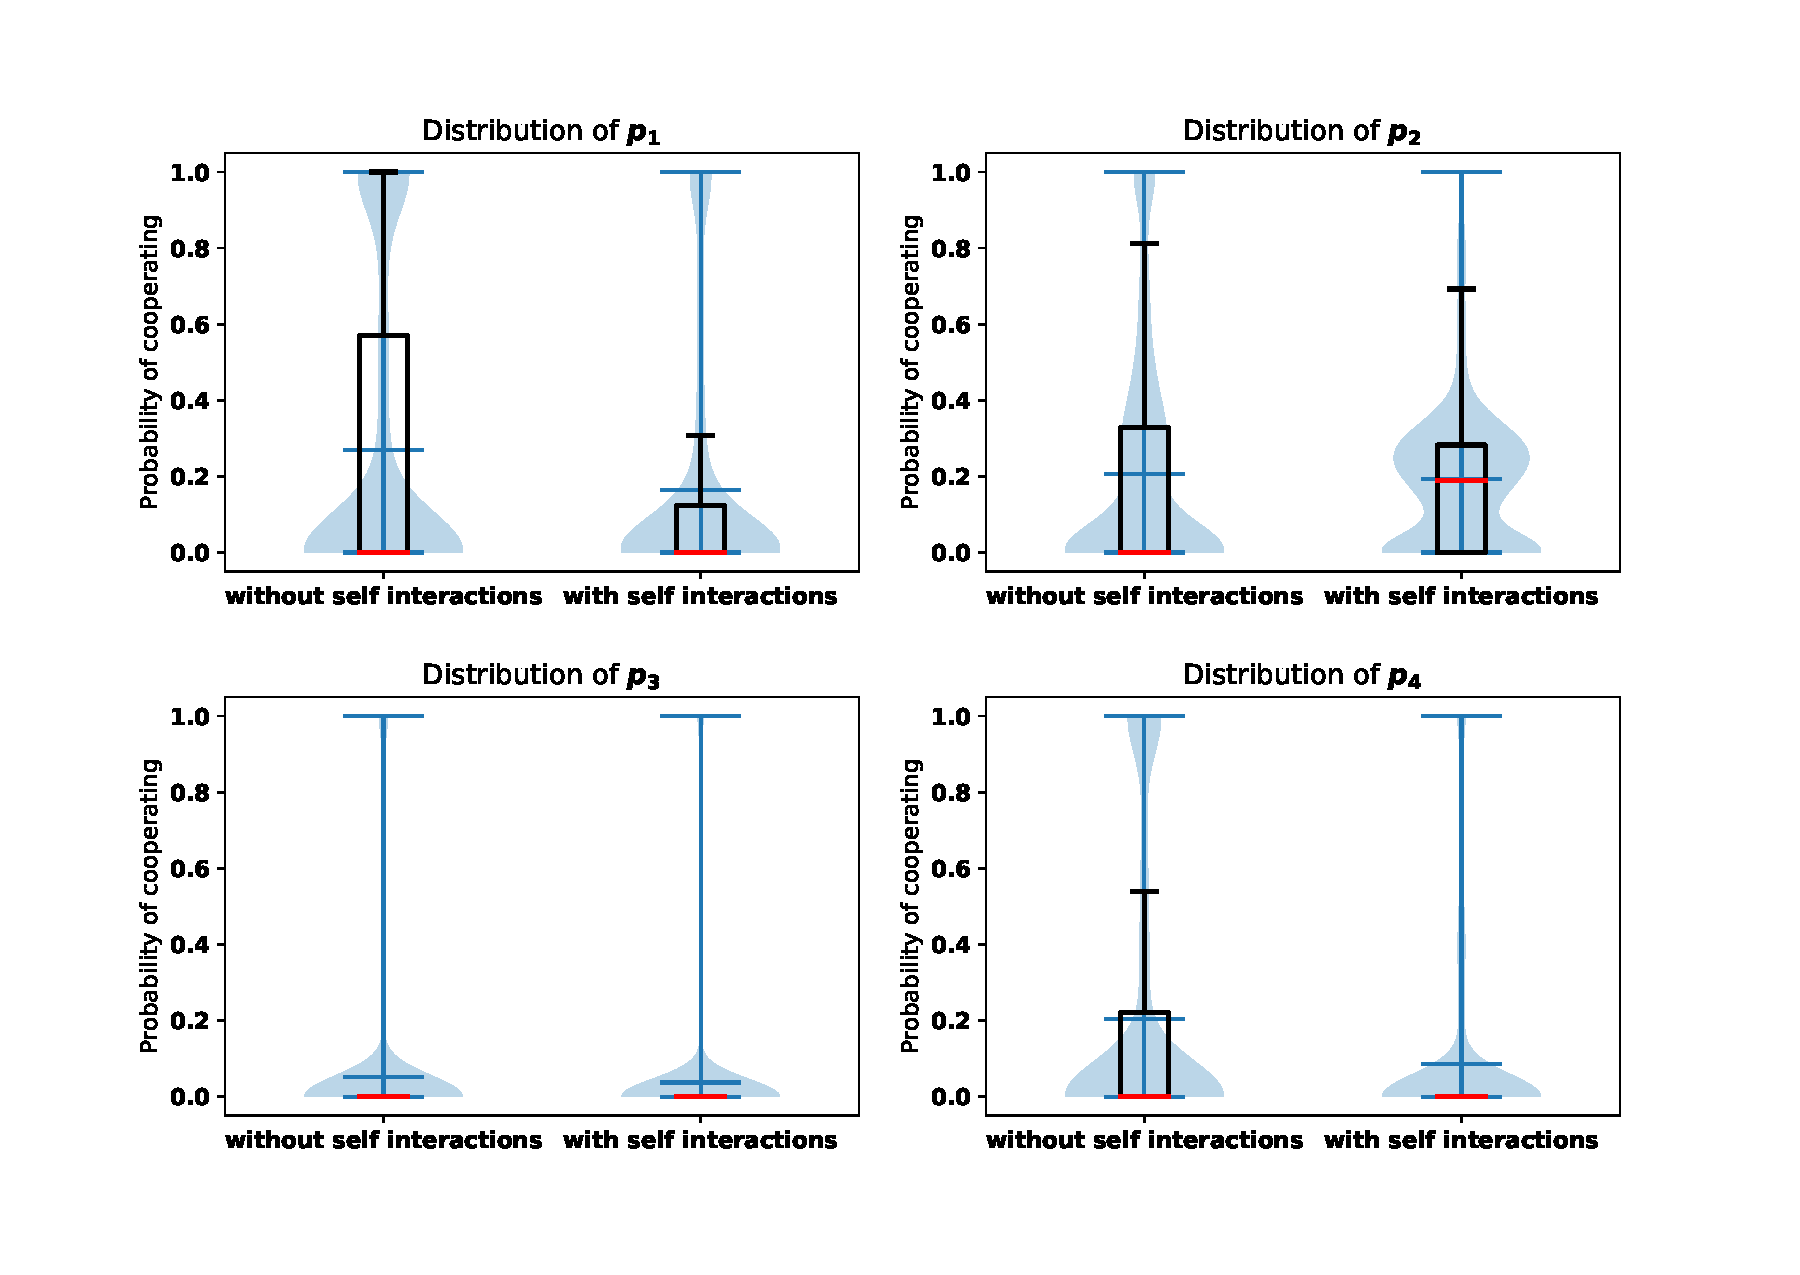
\includegraphics[width=.55\textwidth]{img/behaviour_violin_plots.pdf}
%DIFDELCMD <     %%%
\DIFdelendFL \DIFaddbeginFL 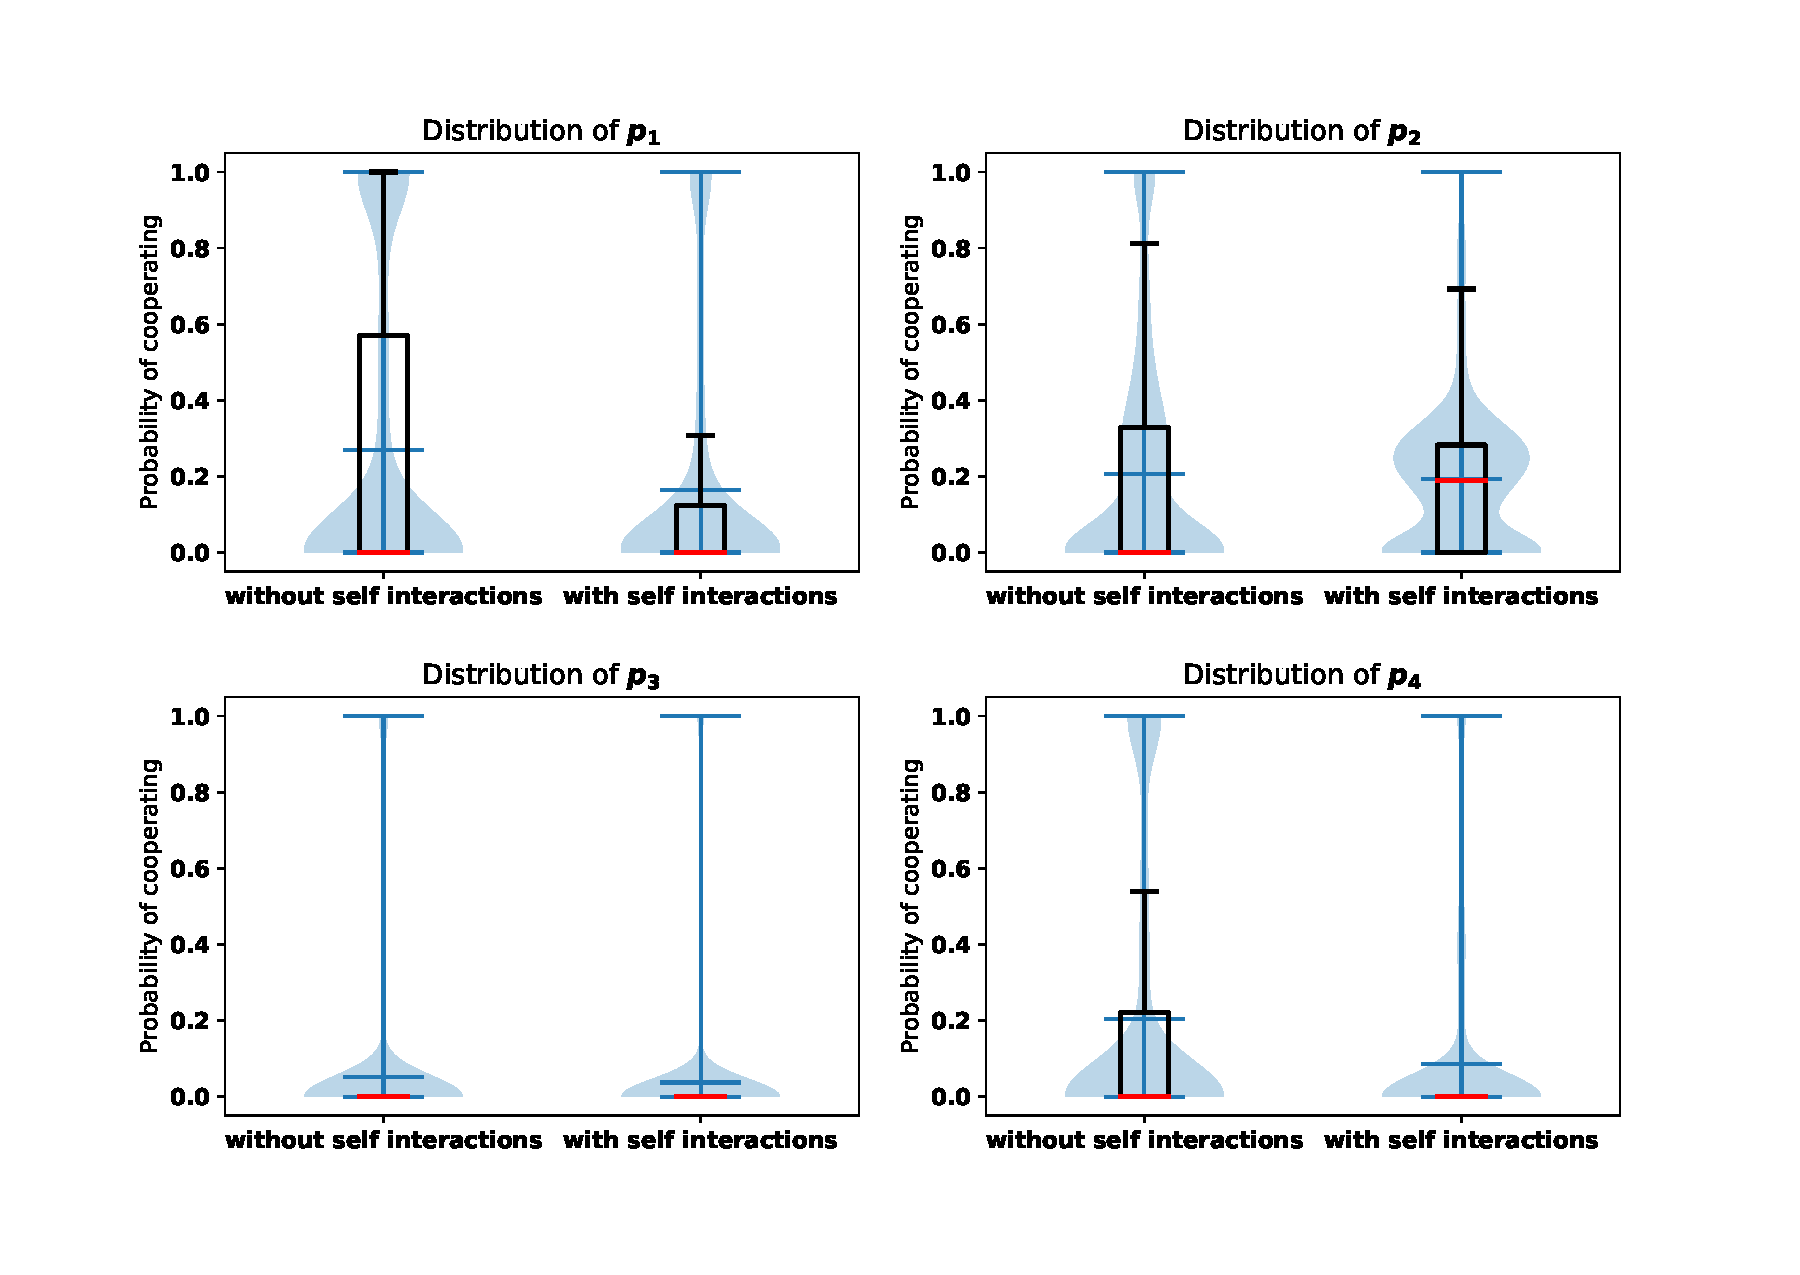
\includegraphics[width=.9\textwidth]{img/behaviour_violin_plots.pdf}
    \DIFaddendFL \caption{Distributions of \(p^*\) for best responses in tournaments and
    evolutionary settings. The medians, denoted as \(\bar{p}^*\), for tournaments
    are \(\bar{p}^* = (0, 0, 0, 0)\), and for evolutionary settings
    \(\bar{p}^* = (0, 0.19, 0, 0)\).}
    \label{fig:behaviour_violin_plots}
\end{figure}

\DIFdelbegin \subsection{\DIFdel{Longer memory best responses}}
%DIFAUXCMD
\addtocounter{subsection}{-1}%DIFAUXCMD
%DIFDELCMD < 

%DIFDELCMD < %%%
\DIFdel{This section focuses on the memory size of strategies. The }\DIFdelend \DIFaddbegin \DIFadd{The other main finding presented in~\mbox{%DIFAUXCMD
\cite{Press20212} }\hspace{0pt}%DIFAUXCMD
was that
short memory of the strategies was all that was needed.
We argue that the second limitation of ZDs in multi opponent
interactions is that of their restricted memory.
To demonstrate the }\DIFaddend effectiveness of memory in the IPD \DIFdelbegin \DIFdel{has been previously explored in the literature,  however, no one
has compared the performance of }\DIFdelend \DIFaddbegin \DIFadd{we explore a best response
}\DIFaddend longer-memory \DIFdelbegin \DIFdel{strategies to }\DIFdelend \DIFaddbegin \DIFadd{strategy against a given set of }\DIFaddend memory-one \DIFaddbegin \DIFadd{opponents,  and compare
it's performance to that of a memory-one }\DIFaddend best \DIFdelbegin \DIFdel{responses}\DIFdelend \DIFaddbegin \DIFadd{response}\DIFaddend .

In~\cite{Harper2017}, a strategy called \textit{Gambler} which makes
probabilistic decisions based on the opponent's \(n_1\) first moves, the
opponent's \(m_1\) last moves and the player's \(m_2\) last moves was
introduced. In this manuscript Gambler with parameters: $n_1 = 2, m_1 = 1$ and $m_2 = 1$ is used
as a longer-memory strategy.
By considering the opponent's first two moves, the opponents last move and the
player's last move, there are only 16 $(4 \times 2 \times 2)$ possible outcomes
that can occur, furthermore, Gambler also makes a probabilistic decision of
cooperating in the opening move. Thus, Gambler is a function \(f: \{\text{C,
D}\} \rightarrow [0, 1]_{\R}\). This can be hard coded as an element
of \([0, 1]_{\R} ^ {16 + 1}\), one probability for each outcome plus the opening
move. Hence, compared to Eq.~\ref{eq:mo_tournament_optimisation}, finding an
optimal Gambler is a 17 dimensional problem given by:

\begin{equation}\label{eq:gambler_optimisation}
    \begin{aligned}
    \max_p: & \ \sum_{i=1} ^ {N} {U_q}^{(i)} (f)
    \\
    \text{such that}: & \ f \in \R_{[0, 1]}^{17}
    \end{aligned}
\end{equation}

Note that Eq. \ref{eq:tournament_utility} can not be used here for the utility
of Gambler, and actual simulated players are used. This is done using~\cite{axelrodproject}
with 500 turns and 200 repetitions, moreover, Eq. \ref{eq:gambler_optimisation}
is solved numerically using Bayesian optimisation.

Similarly to previous sections, a large data set has been generated with
instances of an optimal Gambler and a memory-one best response, available
at~\cite{glynatsi2019}. Estimating a best response Gambler (17 dimensions) is
computational more expensive compared to a best response memory-one (4
dimensions). As a result, the analysis of this section is based on a total of
152 trials. \DIFdelbegin \DIFdel{For each trial two }\DIFdelend \DIFaddbegin \DIFadd{As before, for each trial \(N=2\) }\DIFaddend random opponents have been selected.
\DIFdelbegin \DIFdel{The 152 pair
of opponents are a sub set of the opponents used in section~\ref{section:best_response_memory_one}.
}\DIFdelend 

The ratio between Gambler's utility and the best response memory-one strategy's utility has been calculated and its distribution in
given in Fig.~\ref{fig:utilities_gambler_mem_one}.
It is evident from Fig.~\ref{fig:utilities_gambler_mem_one} that
Gambler always performs as well as the best response memory-one strategy and often performs better. There are
no points where the ratio value is less than 1, thus Gambler never performed less
than the best response memory-one strategy and in places outperforms it.
\DIFdelbegin \DIFdel{This seems to be at odd with the
result of~\mbox{%DIFAUXCMD
\cite{Press2012} }\hspace{0pt}%DIFAUXCMD
that against a memory-one opponent having a longer memory
will not give a strategy any
advantage. }\DIFdelend However, against two memory-one opponents Gambler's performance is better than
the optimal memory-one strategy. This is evidence that in the case of \DIFdelbegin \DIFdel{two opponents}\DIFdelend \DIFaddbegin \DIFadd{multiple
opponents, }\DIFaddend having a
shorter memory is limiting.

\begin{figure}[!htbp]
    \centering
    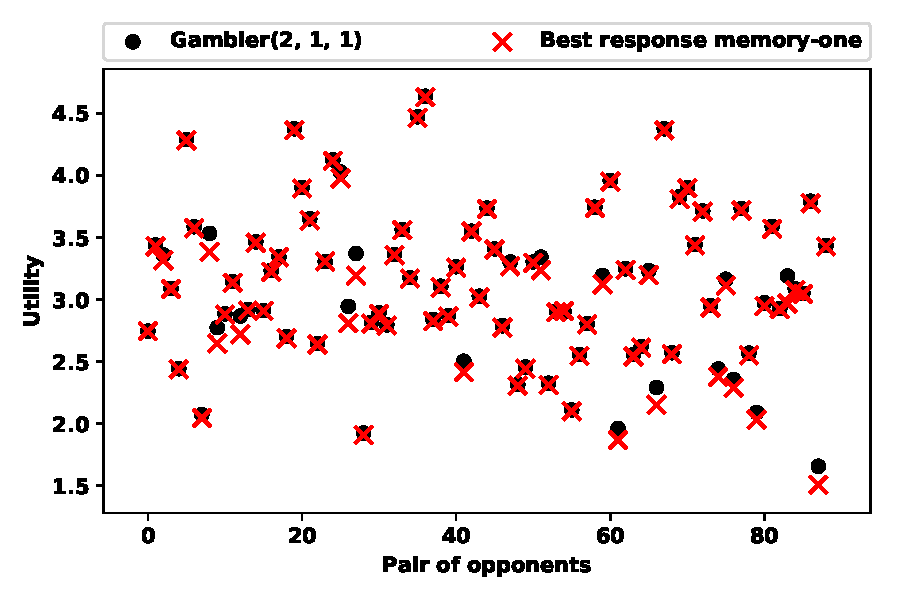
\includegraphics[width=.5\textwidth]{img/gambler_performance_against_mem_one.pdf}
    \caption{The ratio between the utilities of Gambler and best response memory-one
    strategy for 152 different pair of opponents.}\label{fig:utilities_gambler_mem_one}
    %DIF >  TODO Nik: a legend for the lines or a description of the lines in the
    %DIF >  caption?
\end{figure}

\section{Discussion}
This manuscript has considered \textit{best response} strategies in the IPD game, and
more specifically, \textit{memory-one best responses}. It has proven that\DIFdelbegin \DIFdel{there }\DIFdelend \DIFaddbegin \DIFadd{:
}

\begin{itemize}
    \item \DIFadd{The utility
          of a memory-one strategy against a set of memory-one opponents can be written as a sum
          of ratios of quadratic forms (Theorem~\ref{theorem_one}).
    }\item \DIFadd{There }\DIFaddend is a compact way of identifying a memory-one best response to a
        group of opponents \DIFdelbegin \DIFdel{,
and moreover it obtained }\DIFdelend \DIFaddbegin \DIFadd{through a search over a discrete set
        (Theorem~\ref{memone_group_best_response}).
}\end{itemize}

\DIFadd{Note that Theorem~\ref{memone_group_best_response} which does not only have game theoretic
novelty, but also the mathematical novelty of solving quadratic ratio optimisation
problems where the quadratics are non concave.
}

\DIFadd{Moreover Theorem~\ref{theorem_one}, allows us to
obtain }\DIFaddend a condition for which in an environment of memory-one opponents
defection is the stable choice, based only on the coefficients of the opponents\DIFdelbegin \DIFdel{.
The later parts of this paper focused on a series of empirical results , where it
was }\DIFdelend \DIFaddbegin \DIFadd{,
as stated in Lemma~\ref{lemma:stability_of_defection}.
}

\begin{lemma}\label{lemma:stability_of_defection}
    \DIFadd{In a tournament of \(N\) players \(\{q^{(1)}, q^{(2)}, \dots, q^{(N)} \}\)
    for \(q^{(i)} \in \R_{[0, 1]} ^ 4\)
    defection is stable if the transition probabilities of the
    opponents satisfy conditions Eq. \ref{eq:defection_condition_one} and Eq. \ref{eq:defection_condition_two}.
}

    \begin{equation}\label{eq:defection_condition_one}
        \sum_{i=1} ^ N (c^{(i)T} \bar{a}^{(i)} - \bar{c}^{(i)T} a^{(i)}) \leq 0
    \end{equation}

    \DIFadd{while,
}

    \begin{equation}\label{eq:defection_condition_two}
        \sum_{i=1} ^ N \bar{a}^{(i)} \neq 0
    \end{equation}
\end{lemma}

\DIFadd{The proof of Lemma~\ref{lemma:stability_of_defection} is given in
Appendix~\ref{subsection:stability_defection} and a numerical simulation
demonstrating the result is given
in Fig.~\ref{fig:stability_of_defection}.
}

\begin{figure}[!htbp]
    \centering
    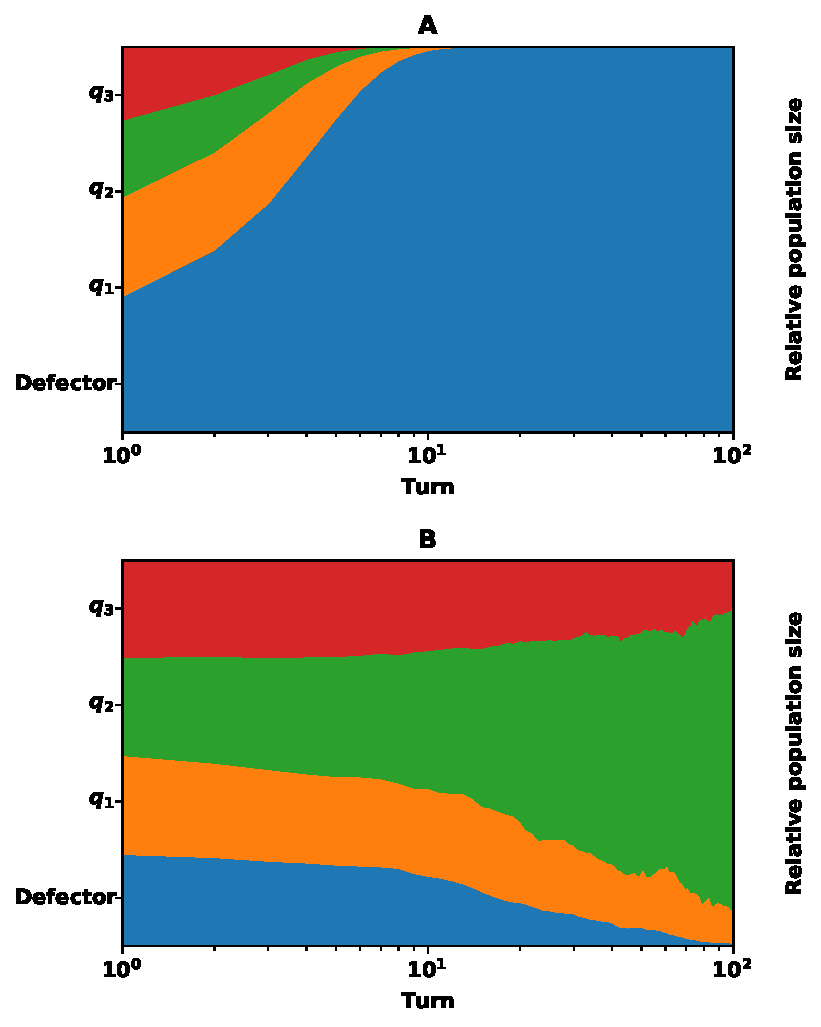
\includegraphics[width=.4\linewidth]{img/stability_of_defection_plots.pdf}
    \caption{\DIFaddFL{A. For \(q_{1}=(0.22199, 0.87073, 0.20672, 0.91861)\),
    $q_{2}=(0.48841, 0.61174, 0.76591, 0.51842)$ and
    $q_{3}=(0.2968, 0.18772, 0.08074, 0.73844)$, Eq.~\ref{eq:defection_condition_one} and
    Eq.~\ref{eq:defection_condition_two} hold and Defector takes over the
    population. B. For $q_{1}=(0.96703, 0.54723, 0.97268, 0.71482)$,
    $q_{2}=(0.69773, 0.21609, 0.97627, 0.0062)$ and
    $q_{3}=(0.25298, 0.43479, 0.77938, 0.19769)$, Eq.~\ref{eq:defection_condition_one} fails
    and Defector does not take over the population.
    These results have been obtained by using~\mbox{%DIFAUXCMD
\cite{axelrodproject} }\hspace{0pt}%DIFAUXCMD
an open
    source research framework for the study of the IPD.}}\label{fig:stability_of_defection}
\end{figure}

\DIFadd{The empirical results have }\DIFaddend shown that the performance and the evolutionary
stability of memory-one strategies rely on adaptability and not on extortion\DIFdelbegin \DIFdel{. Finally,
it was shown }\DIFdelend \DIFaddbegin \DIFadd{,
and }\DIFaddend that memory-one strategies' performance is limited by their memory in cases
where they interact with multiple opponents.

\DIFdelbegin \DIFdel{Following the work described in~\mbox{%DIFAUXCMD
\cite{Nowak1989}}\hspace{0pt}%DIFAUXCMD
, where it was shown that the
utility between two memory-one strategies can be estimated by a Markov
stationary state, we proved that the utilities can be written as a ration of two
quadratic forms in $R^4$, Theorem~\ref{theorem_one}. This was extended to
include multiple opponents, as the IPD is commonly studied in such situations.
This formulation allowed us to introduce an approach for identifying memory-one
best responses to any number of opponents;
Theorem~\ref{memone_group_best_response}. This does not only have game theoretic
novelty, but also a mathematical novelty of solving quadratic ratio optimisation
problems where the quadratics are non concave. The results were used to
define a condition for which defection is known to be stable.
}%DIFDELCMD < 

%DIFDELCMD < %%%
\DIFdel{This manuscript presented several experimental results. All data for the results
is archived in~\mbox{%DIFAUXCMD
\cite{glynatsi2019}}\hspace{0pt}%DIFAUXCMD
. }\DIFdelend These results were mainly to investigate the
behaviour of memory-one strategies and their limitations. A large data set which
contained best responses in tournaments \DIFdelbegin \DIFdel{and in evolutionary settings for $N=2$
was generated }\DIFdelend \DIFaddbegin \DIFadd{whilst including or not self
interactions for \(N=2\)
was generated and is archived in~\mbox{%DIFAUXCMD
\cite{glynatsi2019}}\hspace{0pt}%DIFAUXCMD
}\DIFaddend . This allowed us to investigate their respective behaviours, and
whether it was extortionate acts that made them the most favorable strategies.
\DIFdelbegin \DIFdel{However, it }\DIFdelend \DIFaddbegin \DIFadd{It }\DIFaddend was shown that it was not extortion but adaptability that allowed
the strategies to gain the most from their interactions. In \DIFdelbegin \DIFdel{evolutionary settings it was shown that the best response strategy was even more adaptable, and }\DIFdelend \DIFaddbegin \DIFadd{settings with self interactions
}\DIFaddend there
is some evidence that it is more likely to forgive after being tricked.
\DIFdelbegin \DIFdel{Moreover, the performance of
memory-one strategies was put against the performance of a longer memory
strategy called Gambler. There were several cases where Gambler would outperform
the memory-one strategy, however, a memory-one strategy never managed to
outperform a Gambler. This result occurred whilst considering a Gambler with a
sufficiently larger memory but not a sufficiently larger amount of information
regarding the game.
}\DIFdelend 

All the empirical results presented in this manuscript have been for the case of
$N=2$. In future work we would consider larger values of $N$, however, we
believe that for larger values of $N$ the results that have been presented here
would only be more evident. In addition, we would investigate potential
theoretical results for the \DIFdelbegin \DIFdel{evolutionary }\DIFdelend best responses dynamics algorithm
discussed. \DIFaddbegin \DIFadd{Another interesting avenue would be to study the Moran process with a
dynamically updating best response.
}\DIFaddend 

By specifically exploring the entire \DIFdelbegin \DIFdel{memory space-one }\DIFdelend \DIFaddbegin \DIFadd{space of memory-one }\DIFaddend strategies to identify
the \DIFdelbegin \DIFdel{optimal }\DIFdelend \DIFaddbegin \DIFadd{best }\DIFaddend strategy for a variety of situations, this work \DIFdelbegin \DIFdel{casts }\DIFdelend \DIFaddbegin \DIFadd{adds to the literature
casting }\DIFaddend doubt
on the effectiveness of ZDs, highlights the importance of adaptability and provides
a framework for the continued understanding of these important questions.

\section{Acknowledgements}

A variety of software libraries have been used in this work:

\begin{itemize}
    \item The Axelrod library for IPD simulations~\cite{axelrodproject}.
    \item The Scikit-optimize library for an implementation of Bayesian optimisation~\cite{tim_head_2018_1207017}.
    \item The Matplotlib library for visualisation~\cite{hunter2007matplotlib}.
    \item The SymPy library for symbolic mathematics~\cite{sympy}.
    \item The Numpy library for data manipulation~\cite{walt2011numpy}.
\end{itemize}

% Bibliography
\bibliographystyle{plain}
\bibliography{bibliography.bib}

\section{Appendix}

\subsection{Theorem~\ref{theorem_one} \DIFaddbegin \DIFadd{Proof}\DIFaddend }\DIFdelbegin %DIFDELCMD < \begin{theorem}\label{theorem_one}
%DIFDELCMD < %%%
\DIFdelend \DIFaddbegin \label{appendix:theorem_one}
\DIFaddend 

The \DIFdelbegin \DIFdel{expected }\DIFdelend utility of a \DIFdelbegin \DIFdel{memory-one strategy \(p\in\mathbb{R}_{[0,1]}^4\)
    against a memory-one opponent \(q\in\mathbb{R}_{[0,1]}^4\), denoted
    as }\DIFdelend \DIFaddbegin \DIFadd{memory one player \(p\) against an opponent \(q\), }\DIFaddend \(u_q(p)\),
can be written as a ratio of two quadratic forms \DIFdelbegin \DIFdel{:
}\DIFdelend \DIFaddbegin \DIFadd{on \(R^4\).
}\DIFaddend 

\DIFdelbegin %DIFDELCMD < \begin{equation}\label{eq:optimisation_quadratic}
%DIFDELCMD <     u_q(p) = \frac{\frac{1}{2}pQp^T + cp + a}{\frac{1}{2}p\bar{Q}p^T + \bar{c}p + \bar{a}},
%DIFDELCMD <     \end{equation}
%DIFDELCMD <     %%%
\DIFdel{where \(Q, \bar{Q}\) \(\in \R^{4\times4}\) are square matrices defined by the
    transition probabilities of the opponent \(q_1, q_2, q_3, q_4\) as follows:
}%DIFDELCMD < 

%DIFDELCMD <     \begin{center}
%DIFDELCMD <     \begin{equation}
%DIFDELCMD <     \resizebox{.65\linewidth}{!}{\arraycolsep=2.5pt%
%DIFDELCMD <     \boldmath\(
%DIFDELCMD <     Q = \left[\begin{matrix}0 & 5 q_{4} \left(q_{1} - q_{3}\right) & - q_{4} \left(q_{1} - q_{2}\right) & \left(q_{1} - q_{4}\right) \left(q_{2} - 5 q_{3} - 1\right)\\5 q_{4} \left(q_{1} - q_{3}\right) & 0 & - 3 q_{4} \left(q_{2} - q_{3}\right) & \left(q_{3} - q_{4}\right) \left(5 q_{1} - 3 q_{2} - 2\right)\\- q_{4} \left(q_{1} - q_{2}\right) & - 3 q_{4} \left(q_{2} - q_{3}\right) & 0 & - \left(q_{2} - q_{4}\right) \left(q_{1} - 3 q_{3} - 1\right)\\\left(q_{1} - q_{4}\right) \left(q_{2} - 5 q_{3} - 1\right) & \left(q_{3} - q_{4}\right) \left(5 q_{1} - 3 q_{2} - 2\right) & - \left(q_{2} - q_{4}\right) \left(q_{1} - 3 q_{3} - 1\right) & 0\end{matrix}\right]\)},
%DIFDELCMD <     \end{equation}
%DIFDELCMD <     \begin{equation}\label{eq:q_bar_matrix}
%DIFDELCMD <     \resizebox{.65\linewidth}{!}{\arraycolsep=2.5pt%
%DIFDELCMD <     \boldmath\(
%DIFDELCMD <     \bar{Q} =  \left[\begin{matrix}0 & - \left(q_{1} - q_{3}\right) \left(q_{2} - q_{4} - 1\right) & \left(q_{1} - q_{2}\right) \left(q_{3} - q_{4}\right) & \left(q_{1} - q_{4}\right) \left(q_{2} - q_{3} - 1\right)\\- \left(q_{1} - q_{3}\right) \left(q_{2} - q_{4} - 1\right) & 0 & \left(q_{2} - q_{3}\right) \left(q_{1} - q_{4} - 1\right) & \left(q_{1} - q_{2}\right) \left(q_{3} - q_{4}\right)\\\left(q_{1} - q_{2}\right) \left(q_{3} - q_{4}\right) & \left(q_{2} - q_{3}\right) \left(q_{1} - q_{4} - 1\right) & 0 & - \left(q_{2} - q_{4}\right) \left(q_{1} - q_{3} - 1\right)\\\left(q_{1} - q_{4}\right) \left(q_{2} - q_{3} - 1\right) & \left(q_{1} - q_{2}\right) \left(q_{3} - q_{4}\right) & - \left(q_{2} - q_{4}\right) \left(q_{1} - q_{3} - 1\right) & 0\end{matrix}\right]\)}.
%DIFDELCMD <     \end{equation}
%DIFDELCMD <     \end{center}
%DIFDELCMD < 

%DIFDELCMD <     %%%
\DIFdel{\(c \text{ and } \bar{c}\) \(\in \R^{4 \times 1}\) are similarly defined by:
}%DIFDELCMD < 

%DIFDELCMD <     \begin{equation}\label{eq:q_matrix_numerator}
%DIFDELCMD <     \resizebox{0.25\linewidth}{!}{\arraycolsep=2.5pt%
%DIFDELCMD <     \boldmath\(c = \left[\begin{matrix}- 5 q_{1} q_{4}\\5 q_{4} \left(q_{3} - 1\right)\\q_{4} \left(2 q_{2} + 1\right)\\5 q_{1} q_{4} - 2 q_{2} q_{4} - q_{2} - 5 q_{3} q_{4} + 5 q_{3} - 3 q_{4} + 1\end{matrix}\right]\),}
%DIFDELCMD <     \end{equation}
%DIFDELCMD <     \begin{equation}\label{eq:q_matrix_denominator}
%DIFDELCMD <     \resizebox{0.25\linewidth}{!}{\arraycolsep=2.5pt%
%DIFDELCMD <     \boldmath\(\bar{c} = \left[\begin{matrix}q_{1} \left(q_{2} - q_{4} - 1\right)\\- \left(q_{3} - 1\right) \left(q_{2} - q_{4} - 1\right)\\- q_{1} q_{2} + q_{2} q_{3} + q_{2} - q_{3} + q_{4}\\q_{1} q_{4} - q_{2} - q_{3} q_{4} + q_{3} - q_{4} + 1\end{matrix}\right]\),
%DIFDELCMD <     }
%DIFDELCMD <     \end{equation}
%DIFDELCMD <     %%%
\DIFdel{and the constant terms \(a, \bar{a}\) are defined as \(a = 5 q_{4}\) and
    \(\bar{a} = - q_{2} + q_{4} + 1\).
}%DIFDELCMD < \end{theorem}
%DIFDELCMD < 

%DIFDELCMD < %%%
\DIFdelend \begin{proof}

    It was discussed that \(u_q(p)\) it is the product of the steady \DIFdelbegin \DIFdel{states }\DIFdelend \DIFaddbegin \DIFadd{state
    vector }\DIFaddend \(v\) and the PD payoffs,

    \[u_q(p) = v \cdot (R, S, T, P).\]

    \DIFdelbegin \DIFdel{More specifically, with \((R, P, S, T) = (3, 1, 0, 5)\)
    }\DIFdelend \DIFaddbegin \DIFadd{The steady state vector which is the solution to \(vM = v\) is given by
    }\begingroup
    \tiny
    \begin{equation*}
    \begin{split}
        v =  & \left[ \frac{p_{2} p_{3} (q_{2} q_{4} - q_{3} q_{4}) + p_{2} p_{4} (q_{2} q_{3} - q_{2} q_{4} - q_{3} + q_{4}) +
        p_{3} p_{4} (- q_{2} q_{3} + q_{3} q_{4}) - p_{3} q_{2} q_{4} + p_{4}q_{4} (q_{2} - 1)}{\bar{v}} \right., \\
        & \left. \frac{p_{1} p_{3} (q_{1} q_{4} - q_{2} q_{4}) + p_{1} p_{4} (- q_{1} q_{2} + q_{1} + q_{2} q_{4} -
        q_{4}) + p_{3} p_{4} (q_{1} q_{2} - q_{1} q_{4} - q_{2} + q_{4}) + p_{3}q_{4} (q_{2} - 1) -
         p_{4} q_{2} (q_{4} + 1) + p_{4} (q_{4} - 1)}{\bar{v}} \right., \\
        & \left. \frac{- p_{1} p_{2} (q_{1} q_{4} - q_{3} q_{4}) - p_{1} p_{4} (- q_{1} q_{3} + q_{3} q_{4})
          + p_{1} q_{1} q_{4} - p_{2} p_{4} (q_{1} q_{3} - q_{1} q_{4} - q_{3} + q_{4}) -
          p_{2} q_{4} (q_{3}  + 1) - p_{4}q_{4} (q_{1} + q_{3}) - p_{4} (q_{3}
          + q_{4}) - q_{4}}{\bar{v}} \right., \\ 
        & \left. \frac{p_{1} p_{2} (q_{1} q_{2} - q_{1} - q_{2} q_{3} + q_{3}) + p_{1} p_{3} (- q_{1} q_{3} + q_{2} q_{3})
         - p_{1} q_{1} (q_{2} + 1) + p_{2} p_{3} (- q_{1} q_{2} + q_{1} q_{3}
         + q_{2} - q_{3}) + p_{2} (q_{3}q_{2}  - q_{2} - q_{3} - 1) +
          p_{3} (q_{1} q_{2} - q_{3}q_{2} - q_{2} - q_{3}) + q_{2} - 1}{\bar{v}}\right],
    \end{split}
    \end{equation*}
    \endgroup
\DIFaddend 

    \DIFaddbegin \DIFadd{where,
    }\DIFaddend \begingroup
    \footnotesize
    \DIFdelbegin %DIFDELCMD < \begin{equation}
%DIFDELCMD <         u_q(p) =
%DIFDELCMD <         \left(
%DIFDELCMD <           \frac
%DIFDELCMD <             {\parbox{6in}{$
%DIFDELCMD <                 p_{1} p_{2} (q_{1} q_{2} - 5 q_{1} q_{4} - q_{1} - q_{2} q_{3} + 5 q_{3} q_{4} + q_{3}) + p_{1} p_{3} (- q_{1} q_{3} + q_{2} q_{3}) + p_{1} p_{4} (5 q_{1} q_{3} - 5 q_{3} q_{4}) + p_{3} p_{4} (- 3 q_{2} q_{3} + 3 q_{3} q_{4}) +$ \\
%DIFDELCMD <                 \hspace*{1cm} $ p_{2} p_{3} (- q_{1} q_{2} + q_{1} q_{3} + 3 q_{2} q_{4} + q_{2} - 3 q_{3} q_{4} - q_{3}) + p_{2} p_{4} (- 5 q_{1} q_{3} + 5 q_{1} q_{4} + 3 q_{2} q_{3} - 3 q_{2} q_{4} + 2 q_{3} - 2 q_{4}) + $ \\
%DIFDELCMD <                 \hspace*{1cm} $ p_{1} (- q_{1} q_{2} + 5 q_{1} q_{4} + q_{1}) + p_{2} (q_{2} q_{3} - q_{2} - 5 q_{3} q_{4} - q_{3} + 5 q_{4} + 1) + p_{3} (q_{1} q_{2} - q_{2} q_{3} - 3 q_{2} q_{4} - q_{2} + q_{3}) +$ \\
%DIFDELCMD <                 \hspace*{4cm} $ p_{4} (- 5 q_{1} q_{4} + 3 q_{2} q_{4} + 5 q_{3} q_{4} - 5 q_{3} + 2 q_{4}) + q_{2} - 5 q_{4} - 1$
%DIFDELCMD <             }}
%DIFDELCMD <             {\parbox{6in}{$
%DIFDELCMD <             p_{1} p_{2} (q_{1} q_{2} - q_{1} q_{4} - q_{1} - q_{2} q_{3} + q_{3} q_{4} + q_{3}) + p_{1} p_{3} (- q_{1} q_{3} + q_{1} q_{4} + q_{2} q_{3} - q_{2} q_{4}) + p_{1} p_{4} (- q_{1} q_{2} + q_{1} q_{3} + q_{1} + q_{2} q_{4} - q_{3} q_{4} - q_{4}) +$ \\
%DIFDELCMD <             $ p_{2} p_{3} (- q_{1} q_{2} + q_{1} q_{3} + q_{2} q_{4} + q_{2} - q_{3} q_{4} - q_{3}) + p_{2} p_{4} (- q_{1} q_{3} + q_{1} q_{4} + q_{2} q_{3} - q_{2} q_{4}) + p_{3} p_{4} (q_{1} q_{2} - q_{1} q_{4} - q_{2} q_{3} - q_{2} + q_{3} q_{4} + q_{4}) + $ \\
%DIFDELCMD <             $ p_{1} (- q_{1} q_{2} + q_{1} q_{4} + q_{1}) + p_{2} (q_{2} q_{3} - q_{2} - q_{3} q_{4} - q_{3} + q_{4} + 1) + p_{3} (q_{1} q_{2} - q_{2} q_{3} - q_{2} + q_{3} - q_{4}) + p_{4} (- q_{1} q_{4} + q_{2} + q_{3} q_{4} - q_{3} + q_{4} - 1) + $ \\
%DIFDELCMD <             \hspace*{7cm} $q_{2} - q_{4} - 1$
%DIFDELCMD <           }}
%DIFDELCMD <         \right).
%DIFDELCMD <     \end{equation}%%%
\DIFdelend \DIFaddbegin \begin{equation*}
        \begin{split}
           \bar{v} = & \quad p_{1} p_{2} (q_{1} q_{2} - q_{1} q_{4} - q_{1} - q_{2} q_{3} + q_{3} q_{4} + q_{3}) - p_{1} p_{3} (q_{1} q_{3} - q_{1} q_{4} - q_{2} q_{3} + q_{2} q_{4}) -
           p_{1} p_{4} (q_{1} q_{2} - q_{1} q_{3} - q_{1} - q_{2} q_{4} + q_{3} q_{4} + q_{4}) - \\
           & \quad p_{1} q_{1} (q_{2} + q_{4} + 1) + p_{2} p_{3} (- q_{1} q_{2} + q_{1} q_{3} + q_{2} q_{4} + q_{2} - q_{3} q_{4} - q_{3})
           + p_{2} p_{4} (- q_{1} q_{3} + q_{1} q_{4} + q_{2} q_{3} - q_{2} q_{4}) + p_{2} q_{2} (q_{3} - 1) - p_{2} q_{3} (q_{4} - 1) + \\
           & \quad p_{2} (q_{4} + 1) +  p_{3} p_{4} (q_{1} q_{2} - q_{1} q_{4} - q_{2} q_{3} - q_{2} + q_{3} q_{4} + q_{4}) + p_{3} q_{2} q_{1} ( - p_{3} - 1) + p_{3} (q_{3} -
           q_{4}) - p_{4} (q_{1} q_{4} + q_{2} + q_{3} q_{4} - q_{3} + q_{4} - 1) + \\
           & \quad q_{2} - q_{4} - 1
        \end{split}
        \end{equation*}\DIFaddend 
    \endgroup

    \DIFaddbegin \DIFadd{The dot product of \(v \cdot (R, S, T, P)\) gives,
}

    \begingroup
    \scriptsize
    \begin{equation*}
    \begin{split}
        u_q(p) = & \frac{R \left(p_{2} p_{3} (q_{2} q_{4} - q_{3} q_{4}) + p_{2} p_{4} (q_{2} q_{3} - q_{2} q_{4} - q_{3} + q_{4}) +
        p_{3} p_{4} (- q_{2} q_{3} + q_{3} q_{4}) - p_{3} q_{2} q_{4} + p_{4}q_{4} (q_{2} - 1)\right)}{\bar{v}}  +  \\
        & \frac{S \left(p_{1} p_{3} (q_{1} q_{4} - q_{2} q_{4}) + p_{1} p_{4} (- q_{1} q_{2} + q_{1} + q_{2} q_{4} -
        q_{4}) + p_{3} p_{4} (q_{1} q_{2} - q_{1} q_{4} - q_{2} + q_{4}) + p_{3}q_{4} (q_{2} - 1) -
         p_{4} q_{2} (q_{4} + 1) + p_{4} (q_{4} - 1)\right)}{\bar{v}} + \\
        & \frac{T \left(- p_{1} p_{2} (q_{1} q_{4} - q_{3} q_{4}) - p_{1} p_{4} (- q_{1} q_{3} + q_{3} q_{4})
          + p_{1} q_{1} q_{4} - p_{2} p_{4} (q_{1} q_{3} - q_{1} q_{4} - q_{3} + q_{4}) -
          p_{2} q_{4} (q_{3}  + 1) - p_{4}q_{4} (q_{1} + q_{3}) - p_{4} (q_{3}
          + q_{4}) - q_{4}\right)}{\bar{v}} + \\ 
        & \frac{P \left(p_{1} (p_{2} (q_{1} q_{2} - q_{1} - q_{2} q_{3} + q_{3}) + p_{3} (- q_{1} q_{3} + q_{2} q_{3})
        - q_{1} (q_{2} + 1)) + p_{2} p_{3} ((- q_{1} q_{2} + q_{1} q_{3}
        + q_{2} - q_{3}) + (q_{3}q_{2}  - q_{2} - q_{3} - 1))\right)}{\bar{v}} + \\
        & \frac{P \left(p_{3} (q_{1} q_{2} - q_{3}q_{2} - q_{2} - q_{3}) + q_{2} - 1\right)}{\bar{v}} \implies \\
    \end{split}
    \end{equation*}
    \endgroup

    \begingroup
    \scriptsize
    \begin{equation*}
        u_q(p) =
        \left(
          \frac
            {\parbox{6in}{$ - p_{1} p_{2} (q_{1} - q_{3}) (P q_{2} - P - T q_{4}) + p_{1} p_{3} (q_{1} - q_{2}) (P q_{3} - S q_{4}) + p_{1} p_{4} (q_{1} - q_{4}) (S q_{2} - S - T q_{3}) + p_{2} p_{3} (q_{2} - q_{3}) (P q_{1} - P - R q_{4}) - $ \\
            $ p_{2} p_{4} (q_{3} - q_{4}) (R q_{2} - R - T q_{1} + T) + p_{3} p_{4} (q_{2} - q_{4}) (R q_{3} - S q_{1} + S) + p_{1} q_{1} (P q_{2} - P - T q_{4}) - p_{2} (q_{3} - 1) (P q_{2} - P - T q_{4}) + $ \\
            $ p_{3} (- P q_{1} q_{2} + P q_{2} q_{3} + P q_{2} - P q_{3} + R q_{2} q_{4} - S q_{2} q_{4} + S q_{4}) + p_{4} (- R q_{2} q_{4} + R q_{4} + S q_{2} q_{4} - S q_{2} - S q_{4} + S + T q_{1} q_{4} - T q_{3} q_{4} + T q_{3} - T q_{4}) $ \\
            \hspace*{6.7cm} $- P q_{2} + P + T q_{4}$
            }}
            {\parbox{6in}{$
            p_{1} p_{2} (q_{1} q_{2} - q_{1} q_{4} - q_{1} - q_{2} q_{3} + q_{3} q_{4} + q_{3}) + p_{1} p_{3} (- q_{1} q_{3} + q_{1} q_{4} + q_{2} q_{3} - q_{2} q_{4}) + p_{1} p_{4} (- q_{1} q_{2} + q_{1} q_{3} + q_{1} + q_{2} q_{4} - q_{3} q_{4} - q_{4}) +$ \\
            $ p_{2} p_{3} (- q_{1} q_{2} + q_{1} q_{3} + q_{2} q_{4} + q_{2} - q_{3} q_{4} - q_{3}) + p_{2} p_{4} (- q_{1} q_{3} + q_{1} q_{4} + q_{2} q_{3} - q_{2} q_{4}) + p_{3} p_{4} (q_{1} q_{2} - q_{1} q_{4} - q_{2} q_{3} - q_{2} + q_{3} q_{4} + q_{4}) + $ \\
            $ p_{1} (- q_{1} q_{2} + q_{1} q_{4} + q_{1}) + p_{2} (q_{2} q_{3} - q_{2} - q_{3} q_{4} - q_{3} + q_{4} + 1) + p_{3} (q_{1} q_{2} - q_{2} q_{3} - q_{2} + q_{3} - q_{4}) + p_{4} (- q_{1} q_{4} + q_{2} + q_{3} q_{4} - q_{3} + q_{4} - 1) + $ \\
            \hspace*{7cm} $q_{2} - q_{4} - 1$
          }}
        \right).
    \end{equation*}
    \endgroup

    \DIFaddend Let us consider the numerator of \(u_q(p)\). The cross product terms
    \(p_ip_j\) are given by,

    \begingroup
    \footnotesize
    \DIFdelbegin %DIFDELCMD < \begin{align*}
%DIFDELCMD <     p_{1} p_{2} (q_{1} q_{2} - 5 q_{1} q_{4} - q_{1} - q_{2} q_{3} + 5 q_{3} q_{4}
%DIFDELCMD <     + q_{3}) + p_{1} p_{3} (- q_{1} q_{3} + q_{2} q_{3}) + p_{1} p_{4} (5 q_{1} q_{3} -
%DIFDELCMD <     5 q_{3} q_{4}) + p_{3} p_{4} (- 3 q_{2} q_{3} + 3 q_{3} q_{4}) +  \\
%DIFDELCMD <     p_{2} p_{3} (- q_{1} q_{2} + q_{1} q_{3} + 3 q_{2} q_{4} + q_{2} - 3 q_{3} q_{4} - q_{3}) +
%DIFDELCMD <     p_{2} p_{4} (- 5 q_{1} q_{3} + 5 q_{1} q_{4} + 3 q_{2} q_{3} - 3 q_{2} q_{4} +
%DIFDELCMD <     2 q_{3} - 2 q_{4}).
%DIFDELCMD <     \end{align*}%%%
\DIFdelend \DIFaddbegin \begin{align*}
    - p_{1} p_{2} (q_{1} - q_{3}) (P q_{2} - P - T q_{4}) + p_{1} p_{3} (q_{1} - q_{2}) (P q_{3} - S q_{4}) + p_{1} p_{4} (q_{1} - q_{4}) (S q_{2} - S - T q_{3}) + \\
    p_{2} p_{3} (q_{2} - q_{3}) (P q_{1} - P - R q_{4}) - p_{2} p_{4} (q_{3} - q_{4}) (R q_{2} - R - T q_{1} + T) + p_{3} p_{4} (q_{2} - q_{4}) (R q_{3} - S q_{1} + S)
    \end{align*}\DIFaddend 
    \endgroup

    This can be re written in a matrix format given by
    Eq.~\ref{eq:cross_product_coeffs}.

    \DIFdelbegin %DIFDELCMD < \begin{equation}\label{eq:cross_product_coeffs}
%DIFDELCMD <         \resizebox{0.8\linewidth}{!}{\arraycolsep=2.5pt%
%DIFDELCMD <         \boldmath%
\mbox{%DIFAUXCMD
\( 
%DIFDELCMD <         (p_1, p_2, p_3, p_4) \frac{1}{2} \left[\begin{matrix}0 & 5 q_{4} \left(q_{1} - q_{3}\right) & - q_{4} \left(q_{1} - q_{2}\right) & \left(q_{1} - q_{4}\right) \left(q_{2} - 5 q_{3} - 1\right)\\5 q_{4} \left(q_{1} - q_{3}\right) & 0 & - 3 q_{4} \left(q_{2} - q_{3}\right) & \left(q_{3} - q_{4}\right) \left(5 q_{1} - 3 q_{2} - 2\right)\\- q_{4} \left(q_{1} - q_{2}\right) & - 3 q_{4} \left(q_{2} - q_{3}\right) & 0 & - \left(q_{2} - q_{4}\right) \left(q_{1} - 3 q_{3} - 1\right)\\\left(q_{1} - q_{4}\right) \left(q_{2} - 5 q_{3} - 1\right) & \left(q_{3} - q_{4}\right) \left(5 q_{1} - 3 q_{2} - 2\right) & - \left(q_{2} - q_{4}\right) \left(q_{1} - 3 q_{3} - 1\right) & 0\end{matrix}\right] \begin{pmatrix} 
%DIFDELCMD <         p_1 \\
%DIFDELCMD <         p_2 \\
%DIFDELCMD <         p_3 \\
%DIFDELCMD <         p_4 \end{pmatrix}
%DIFDELCMD <
\)
}%DIFAUXCMD

%DIFDELCMD <     \end{equation}%%%
\DIFdelend \DIFaddbegin \begin{equation}\label{eq:cross_product_coeffs}
        \resizebox{0.9\linewidth}{!}{\arraycolsep=2.5pt%
        \boldmath%
\mbox{%DIFAUXCMD
\(
        (p_1, p_2, p_3, p_4) \frac{1}{2} \left[\begin{matrix}0 & 5 q_{4} \left(q_{1} - q_{3}\right) & - q_{4} \left(q_{1} - q_{2}\right) & \left(q_{1} - q_{4}\right) \left(q_{2} - 5 q_{3} - 1\right)\\5 q_{4} \left(q_{1} - q_{3}\right) & 0 & - 3 q_{4} \left(q_{2} - q_{3}\right) & \left(q_{3} - q_{4}\right) \left(5 q_{1} - 3 q_{2} - 2\right)\\- q_{4} \left(q_{1} - q_{2}\right) & - 3 q_{4} \left(q_{2} - q_{3}\right) & 0 & - \left(q_{2} - q_{4}\right) \left(q_{1} - 3 q_{3} - 1\right)\\\left(q_{1} - q_{4}\right) \left(q_{2} - 5 q_{3} - 1\right) & \left(q_{3} - q_{4}\right) \left(5 q_{1} - 3 q_{2} - 2\right) & - \left(q_{2} - q_{4}\right) \left(q_{1} - 3 q_{3} - 1\right) & 0\end{matrix}\right] \begin{pmatrix}
        p_1 \\
        p_2 \\
        p_3 \\
        p_4 \end{pmatrix}
        \)
}%DIFAUXCMD
}
    \end{equation}\DIFaddend 

    Similarly, the linear terms are given by,

    \begingroup
    \footnotesize
    \DIFdelbegin %DIFDELCMD < \begin{align*}
%DIFDELCMD <     p_{1} (- q_{1} q_{2} + 5 q_{1} q_{4} + q_{1}) + p_{2} (q_{2} q_{3} - q_{2} - 5 q_{3} q_{4} - q_{3} + 5 q_{4} + 1) + p_{3} (q_{1} q_{2} - q_{2} q_{3} - 3 q_{2} q_{4} - q_{2} + q_{3}) + \\
%DIFDELCMD <     p_{4} (- 5 q_{1} q_{4} + 3 q_{2} q_{4} + 5 q_{3} q_{4} - 5 q_{3} + 2 q_{4}).
%DIFDELCMD <     \end{align*}%%%
\DIFdelend \DIFaddbegin \begin{align*}
    p_{1} q_{1} (P q_{2} - P - T q_{4}) - p_{2} & (q_{3} - 1) (P q_{2} - P - T q_{4}) + p_{3} (- P q_{1} q_{2} + P q_{2} q_{3} + P q_{2} - P q_{3} + R q_{2} q_{4} - S q_{2} q_{4} + S q_{4}) + \\
    p_{4} & (- R q_{2} q_{4} + R q_{4} + S q_{2} q_{4} - S q_{2} - S q_{4} + S + T q_{1} q_{4} - T q_{3} q_{4} + T q_{3} - T q_{4})
    \end{align*}\DIFaddend 
    \endgroup

    and the expression can be written using a matrix format as
    Eq.~\ref{eq:linear_coeffs}.

    \DIFdelbegin %DIFDELCMD < \begin{equation}\label{eq:linear_coeffs}
%DIFDELCMD <         \resizebox{0.38\linewidth}{!}{\arraycolsep=2.5pt%
%DIFDELCMD <         \boldmath\(
%DIFDELCMD <         (p_1, p_2, p_3, p_4) \left[\begin{matrix}- 5 q_{1} q_{4}\\5 q_{4} \left(q_{3} - 1\right)\\q_{4} \left(2 q_{2} + 1\right)\\5 q_{1} q_{4} - 2 q_{2} q_{4} - q_{2} - 5 q_{3} q_{4} + 5 q_{3} - 3 q_{4} + 1\end{matrix}\right]\)}
%DIFDELCMD <     \end{equation}%%%
\DIFdelend \DIFaddbegin \begin{equation}\label{eq:linear_coeffs}
        \resizebox{0.60\linewidth}{!}{\arraycolsep=2.5pt%
        \boldmath\(
        (p_1, p_2, p_3, p_4) \left[\begin{matrix}- 5 q_{1} q_{4}\\5 q_{4} \left(q_{3} - 1\right)\\q_{4} \left(2 q_{2} + 1\right)\\5 q_{1} q_{4} - 2 q_{2} q_{4} - q_{2} - 5 q_{3} q_{4} + 5 q_{3} - 3 q_{4} + 1\end{matrix}\right]\)}
    \end{equation}\DIFaddend 

    Finally, the constant term of the numerator, which is obtained by
    substituting $p=(0, 0, 0, 0)$, is given by Eq.~\ref{eq:constant}.

    \DIFdelbegin %DIFDELCMD < \begin{equation}\label{eq:constant}
%DIFDELCMD <     q_{2} - 5 q_{4} - 1
%DIFDELCMD <     \end{equation}%%%
\DIFdelend \DIFaddbegin \begin{equation}\label{eq:constant}
    - P q_{2} + P + T q_{4}
    \end{equation}\DIFaddend 

    Combining Eq.~\ref{eq:cross_product_coeffs}, Eq.~\ref{eq:linear_coeffs} and
    Eq.~\ref{eq:constant} gives that the numerator of \(u_q(p)\) can be written
    as,

    \begingroup
    \tiny\boldmath
    \DIFdelbegin %DIFDELCMD < \begin{align*}
%DIFDELCMD <         \frac{1}{2}p & \left[\begin{matrix}0 & 5 q_{4} \left(q_{1} - q_{3}\right) & - q_{4} \left(q_{1} - q_{2}\right) & \left(q_{1} - q_{4}\right) \left(q_{2} - 5 q_{3} - 1\right)\\5 q_{4} \left(q_{1} - q_{3}\right) & 0 & - 3 q_{4} \left(q_{2} - q_{3}\right) & \left(q_{3} - q_{4}\right) \left(5 q_{1} - 3 q_{2} - 2\right)\\- q_{4} \left(q_{1} - q_{2}\right) & - 3 q_{4} \left(q_{2} - q_{3}\right) & 0 & - \left(q_{2} - q_{4}\right) \left(q_{1} - 3 q_{3} - 1\right)\\\left(q_{1} - q_{4}\right) \left(q_{2} - 5 q_{3} - 1\right) & \left(q_{3} - q_{4}\right) \left(5 q_{1} - 3 q_{2} - 2\right) & - \left(q_{2} - q_{4}\right) \left(q_{1} - 3 q_{3} - 1\right) & 0\end{matrix}\right] p^T +  \\
%DIFDELCMD <         & \left[\begin{matrix}0 & 5 q_{4} \left(q_{1} - q_{3}\right) & - q_{4} \left(q_{1} - q_{2}\right) & \left(q_{1} - q_{4}\right) \left(q_{2} - 5 q_{3} - 1\right)\\5 q_{4} \left(q_{1} - q_{3}\right) & 0 & - 3 q_{4} \left(q_{2} - q_{3}\right) & \left(q_{3} - q_{4}\right) \left(5 q_{1} - 3 q_{2} - 2\right)\\- q_{4} \left(q_{1} - q_{2}\right) & - 3 q_{4} \left(q_{2} - q_{3}\right) & 0 & - \left(q_{2} - q_{4}\right) \left(q_{1} - 3 q_{3} - 1\right)\\\left(q_{1} - q_{4}\right) \left(q_{2} - 5 q_{3} - 1\right) & \left(q_{3} - q_{4}\right) \left(5 q_{1} - 3 q_{2} - 2\right) & - \left(q_{2} - q_{4}\right) \left(q_{1} - 3 q_{3} - 1\right) & 0\end{matrix}\right] p + q_{2} - 5 q_{4} - 1
%DIFDELCMD <     \end{align*}%%%
\DIFdelend \DIFaddbegin \begin{align*}
        \frac{1}{2}p & \left[\begin{matrix}0 & 5 q_{4} \left(q_{1} - q_{3}\right) & - q_{4} \left(q_{1} - q_{2}\right) & \left(q_{1} - q_{4}\right) \left(q_{2} - 5 q_{3} - 1\right)\\5 q_{4} \left(q_{1} - q_{3}\right) & 0 & - 3 q_{4} \left(q_{2} - q_{3}\right) & \left(q_{3} - q_{4}\right) \left(5 q_{1} - 3 q_{2} - 2\right)\\- q_{4} \left(q_{1} - q_{2}\right) & - 3 q_{4} \left(q_{2} - q_{3}\right) & 0 & - \left(q_{2} - q_{4}\right) \left(q_{1} - 3 q_{3} - 1\right)\\\left(q_{1} - q_{4}\right) \left(q_{2} - 5 q_{3} - 1\right) & \left(q_{3} - q_{4}\right) \left(5 q_{1} - 3 q_{2} - 2\right) & - \left(q_{2} - q_{4}\right) \left(q_{1} - 3 q_{3} - 1\right) & 0\end{matrix}\right] p^T +  \\
        & \left[\begin{matrix}- 5 q_{1} q_{4}\\5 q_{4} \left(q_{3} - 1\right)\\q_{4} \left(2 q_{2} + 1\right)\\5 q_{1} q_{4} - 2 q_{2} q_{4} - q_{2} - 5 q_{3} q_{4} + 5 q_{3} - 3 q_{4} + 1\end{matrix}\right] p - P q_{2} + P + T q_{4}
    \end{align*}\DIFaddend 
    \endgroup

    and equivalently as,

    \[\frac{1}{2}pQp^T + cp + a\]

    where \(Q\) \(\in \R^{4\times4}\) is a square matrix defined by the
    transition probabilities of the opponent \(q_1, q_2, q_3, q_4\) as follows:

    \DIFdelbegin %DIFDELCMD < \begin{equation*}
%DIFDELCMD <         \resizebox{0.7\linewidth}{!}{\arraycolsep=2.5pt%
%DIFDELCMD <         \boldmath\(
%DIFDELCMD <         Q = \left[\begin{matrix}0 & 5 q_{4} \left(q_{1} - q_{3}\right) & - q_{4} \left(q_{1} - q_{2}\right) & \left(q_{1} - q_{4}\right) \left(q_{2} - 5 q_{3} - 1\right)\\5 q_{4} \left(q_{1} - q_{3}\right) & 0 & - 3 q_{4} \left(q_{2} - q_{3}\right) & \left(q_{3} - q_{4}\right) \left(5 q_{1} - 3 q_{2} - 2\right)\\- q_{4} \left(q_{1} - q_{2}\right) & - 3 q_{4} \left(q_{2} - q_{3}\right) & 0 & - \left(q_{2} - q_{4}\right) \left(q_{1} - 3 q_{3} - 1\right)\\\left(q_{1} - q_{4}\right) \left(q_{2} - 5 q_{3} - 1\right) & \left(q_{3} - q_{4}\right) \left(5 q_{1} - 3 q_{2} - 2\right) & - \left(q_{2} - q_{4}\right) \left(q_{1} - 3 q_{3} - 1\right) & 0\end{matrix}\right]\)},
%DIFDELCMD <     \end{equation*}%%%
\DIFdelend \DIFaddbegin \begin{equation*}
        \resizebox{0.9\linewidth}{!}{\arraycolsep=2.5pt%
        \boldmath\(
        Q = \left[\begin{matrix}0 & 5 q_{4} \left(q_{1} - q_{3}\right) & - q_{4} \left(q_{1} - q_{2}\right) & \left(q_{1} - q_{4}\right) \left(q_{2} - 5 q_{3} - 1\right)\\5 q_{4} \left(q_{1} - q_{3}\right) & 0 & - 3 q_{4} \left(q_{2} - q_{3}\right) & \left(q_{3} - q_{4}\right) \left(5 q_{1} - 3 q_{2} - 2\right)\\- q_{4} \left(q_{1} - q_{2}\right) & - 3 q_{4} \left(q_{2} - q_{3}\right) & 0 & - \left(q_{2} - q_{4}\right) \left(q_{1} - 3 q_{3} - 1\right)\\\left(q_{1} - q_{4}\right) \left(q_{2} - 5 q_{3} - 1\right) & \left(q_{3} - q_{4}\right) \left(5 q_{1} - 3 q_{2} - 2\right) & - \left(q_{2} - q_{4}\right) \left(q_{1} - 3 q_{3} - 1\right) & 0\end{matrix}\right]\)},
    \end{equation*}\DIFaddend 

    \(c\) \(\in \R^{4 \times 1}\) is similarly defined by:

    \DIFdelbegin %DIFDELCMD < \begin{equation*}
%DIFDELCMD <         \resizebox{0.3\linewidth}{!}{\arraycolsep=2.5pt%
%DIFDELCMD <         \boldmath\(c = \left[\begin{matrix}- 5 q_{1} q_{4}\\5 q_{4} \left(q_{3} - 1\right)\\q_{4} \left(2 q_{2} + 1\right)\\5 q_{1} q_{4} - 2 q_{2} q_{4} - q_{2} - 5 q_{3} q_{4} + 5 q_{3} - 3 q_{4} + 1\end{matrix}\right]\),}
%DIFDELCMD <     \end{equation*}%%%
\DIFdelend \DIFaddbegin \begin{equation*}
        \resizebox{0.55\linewidth}{!}{\arraycolsep=2.5pt%
        \boldmath\(c = \left[\begin{matrix}- 5 q_{1} q_{4}\\5 q_{4} \left(q_{3} - 1\right)\\q_{4} \left(2 q_{2} + 1\right)\\5 q_{1} q_{4} - 2 q_{2} q_{4} - q_{2} - 5 q_{3} q_{4} + 5 q_{3} - 3 q_{4} + 1\end{matrix}\right]\),}
    \end{equation*}\DIFaddend 

    and \(a = 5 q_{4}\).

    The same process is done for the denominator.
\end{proof}

\subsection{Theorem~\ref{memone_group_best_response} \DIFaddbegin \DIFadd{Proof}\DIFaddend }\DIFdelbegin %DIFDELCMD < \begin{theorem}\label{memone_group_best_response}
%DIFDELCMD < 

%DIFDELCMD < %%%
\DIFdelend \DIFaddbegin \label{appendix:memone_group_best_response}
\DIFaddend The optimal behaviour of a memory-one strategy player \(p^* \in \R_{[0, 1]} ^
4\) against a set of \(N\) opponents \(\{q^{(1)}, q^{(2)}, \dots, q^{(N)} \}\)
for \(q^{(i)} \in \R_{[0, 1]} ^ 4\) is given by:

\[p^* = \textnormal{argmax}\sum\limits_{i=1} ^ N  u_q(p), \ p \in S_q.\]

The set \(S_q\) is defined as all the possible combinations of:

\DIFdelbegin %DIFDELCMD < {\scriptsize
%DIFDELCMD < %%%
\DIFdelend \begin{equation}\label{eq:s_q_set}
    S_q =
    \left\{p \in \mathbb{R} ^ 4 \left|
        \begin{aligned}
            \bullet\quad p_j \in \{0, 1\} & \quad \text{and} \quad \frac{d}{dp_k}
            \sum\limits_{i=1} ^ N  u_q^{(i)}(p) = 0 \\
            & \quad \text{for all} \quad j \in J \quad \&  \quad k \in K  \quad \text{for all} \quad J, K \\
            & \quad \text{where} \quad J \cap K = \O \quad
            \text{and} \quad J \cup K = \{1, 2, 3, 4\}.\\
            \bullet\quad  p \in \{0, 1\} ^ 4
        \end{aligned}\right.
    \right\}.
\end{equation}
\DIFdelbegin %DIFDELCMD < }
%DIFDELCMD < %%%
\DIFdelend 

\DIFdelbegin \DIFdel{Note that there is no immediate way to find the zeros of
\(\frac{d}{dp} \sum\limits_{i=1} ^ N  u_q(p)\) where,
}%DIFDELCMD < 

%DIFDELCMD < {\scriptsize
%DIFDELCMD < \begin{align}\label{eq:mo_tournament_derivative}
%DIFDELCMD <     \frac{d}{dp} \sum\limits_{i=1} ^ {N} {u_q}^{(i)} (p) & = \displaystyle\sum\limits_{i=1} ^ {N}
%DIFDELCMD <     \frac{\left(pQ^{(i)} + c^{(i)}\right) \left(\frac{1}{2} p\bar{Q}^{(i)} p^T + \bar{c}^{(i)} p + \bar{a}^ {(i)}\right)}{\left(\frac{1}{2} p\bar{Q}^{(i)} p^T + \bar{c}^{(i)} p + \bar{a}^ {(i)}\right)^ 2}
%DIFDELCMD <     - \frac{\left(p\bar{Q}^{(i)} + \bar{c}^{(i)}\right) \left(\frac{1}{2} pQ^{(i)} p^T + c^{(i)} p + a^ {(i)}\right)}{\left(\frac{1}{2} p\bar{Q}^{(i)} p^T + \bar{c}^{(i)} p + \bar{a}^ {(i)}\right)^ 2}
%DIFDELCMD < \end{align}
%DIFDELCMD < }
%DIFDELCMD < 

%DIFDELCMD < %%%
\DIFdel{For \(\frac{d}{dp} \sum\limits_{i=1} ^ N  u_q(p)\) to equal zero then:
}%DIFDELCMD < 

%DIFDELCMD < {\scriptsize
%DIFDELCMD < \begin{align}\label{eq:polynomials_roots}
%DIFDELCMD <     \displaystyle\sum\limits_{i=1} ^ {N}
%DIFDELCMD <     \left(pQ^{(i)} + c^{(i)}\right) \left(\frac{1}{2} p\bar{Q}^{(i)} p^T + \bar{c}^{(i)} p + \bar{a}^ {(i)}\right)
%DIFDELCMD <     - \left(p\bar{Q}^{(i)} + \bar{c}^{(i)}\right) \left(\frac{1}{2} pQ^{(i)} p^T + c^{(i)} p + a^ {(i)}\right)
%DIFDELCMD <     & = 0, \quad {while} \\
%DIFDELCMD <     \displaystyle\sum\limits_{i=1} ^ {N} \frac{1}{2} p\bar{Q}^{(i)} p^T + \bar{c}^{(i)} p + \bar{a}^ {(i)} & \neq 0.
%DIFDELCMD < \end{align}}
%DIFDELCMD < 

%DIFDELCMD < \end{theorem}
%DIFDELCMD < 

%DIFDELCMD < %%%
\DIFdelend \begin{proof}
    The \DIFdelbegin \DIFdel{optimal behaviour of a memory-one strategy player
    \(p^* \in \R_{[0, 1]} ^ 4\)
    against a set of \(N\) opponents \(\{q^{(1)}, q^{(2)}, \dots, q^{(N)} \}\)
    for \(q^{(i)} \in \R_{[0, 1]} ^ 4\) is established by:
    }%DIFDELCMD < 

%DIFDELCMD <     \[p^* = \textnormal{argmax}\left(\sum\limits_{i=1} ^ N  u_q(p)\right), \ p \in S_q,\]
%DIFDELCMD <     

%DIFDELCMD <     %%%
\DIFdel{where \(S_q\) is given by:
    }%DIFDELCMD < {\scriptsize
%DIFDELCMD <     \begin{equation}\label{eq:s_q_set}
%DIFDELCMD <         S_q =
%DIFDELCMD <         \left\{p \in \mathbb{R} ^ 4 \left|
%DIFDELCMD <             \begin{aligned}
%DIFDELCMD <                 \bullet\quad p_j \in \{0, 1\} & \quad \text{and} \quad \frac{d}{dp_k} 
%DIFDELCMD <                 \sum\limits_{i=1} ^ N  u_q^{(i)}(p) = 0 \\
%DIFDELCMD <                 & \quad \text{for all} \quad j \in J \quad \&  \quad k \in K  \quad \text{for all} \quad J, K \\
%DIFDELCMD <                 & \quad \text{where} \quad J \cap K = \O \quad
%DIFDELCMD <                 \text{and} \quad J \cup K = \{1, 2, 3, 4\}.\\
%DIFDELCMD <                 \bullet\quad  p \in \{0, 1\} ^ 4
%DIFDELCMD <             \end{aligned}\right.
%DIFDELCMD <         \right\}.
%DIFDELCMD <     \end{equation}}
%DIFDELCMD < 

%DIFDELCMD <     %%%
\DIFdel{The }\DIFdelend optimisation problem of Eq.~\ref{eq:mo_tournament_optimisation}

    \begin{equation}\label{eq:mo_tournament_optimisation}
        \begin{aligned}
        \max_p: & \ \sum_{i=1} ^ {N} {u_q}^{(i)} (p)
        \\
        \text{such that}: & \ p \in \R_{[0, 1]}
        \end{aligned}
    \end{equation}

    can be written as:

    \begin{equation}\label{eq:mo_tournament_optimisation_standard}
        \begin{aligned}
        \max_p: & \ \sum_{i=1} ^ {N} {u_q}^{(i)} (p)
        \\
        \text{such that}: p_i & \leq 1 \text{ for } \in \{1, 2, 3, 4\} \\
        - p_i & \leq 0 \text{ for } \in \{1, 2, 3, 4\} \\
        \end{aligned}
    \end{equation}

    The optimisation problem has two inequality constraints and regarding the
    optimality this means that:

    \begin{itemize}
        \item either the optimum is away from the boundary of the optimization
        domain, and so the constraints plays no role;
        \item or the optimum is on the constraint boundary.
    \end{itemize}

    Thus, the following three cases must be considered:

    \textbf{Case 1:} The solution is on the boundary and any of the possible
    combinations for $p_i \in \{0, 1\}$ for $i \in \{1, 2, 3, 4\}$ are candidate
    optimal solutions.

    \textbf{Case 2:} The optimum is away from the boundary of the optimization
    domain and the interior solution $p^*$ necessarily satisfies the condition
    \(\frac{d}{dp} \sum\limits_{i=1} ^ N  u_q(p^*) = 0\).

    \textbf{Case 3:} The optimum is away from the boundary of the optimization
    domain but some constraints are equalities. The candidate solutions in this
    case are any combinations of $p_j \in \{0, 1\} \quad \text{and} \quad
    \frac{d}{dp_k} \sum\limits_{i=1} ^ N  u_q^{(i)}(p) = 0$ forall $ j \in J
    \text{ \& } k \in K \text{ forall } J, K \text{ where } J \cap K = \O
    \text{ and } J \cup K = \{1, 2, 3, 4\}.$

    Combining cases 1-3 a set of candidate \DIFdelbegin \DIFdel{solution }\DIFdelend \DIFaddbegin \DIFadd{solutions, denoted as \(S_q\), }\DIFaddend is
    constructed as: {\scriptsize
    \begin{equation*}
        S_q =
        \left\{p \in \mathbb{R} ^ 4 \left|
            \begin{aligned}
                \bullet\quad p_j \in \{0, 1\} & \quad \text{and} \quad \frac{d}{dp_k}
                \sum\limits_{i=1} ^ N  u_q^{(i)}(p) = 0
                \quad \text{for all} \quad j \in J \quad \&  \quad k \in K  \quad \text{for all} \quad J, K \\
                & \quad \text{where} \quad J \cap K = \O \quad
                \text{and} \quad J \cup K = \{1, 2, 3, 4\}.\\
                \bullet\quad  p \in \{0, 1\} ^ 4
            \end{aligned}\right.
        \right\}.
    \end{equation*}}

    \DIFdelbegin \DIFdel{This set is denoted as $S_q$ and the }\DIFdelend \DIFaddbegin \DIFadd{The derivative of \(\sum\limits_{i=1} ^ N  u_q^{(i)}(p)\) calculated using
    the following property (see~\mbox{%DIFAUXCMD
\cite{Abadir2005} }\hspace{0pt}%DIFAUXCMD
for details):
}

    \begin{equation}\label{eq:first_derivative_property}
    \frac{d x A x^T}{dx} =  2Ax.
    \end{equation}

    \DIFadd{Using property~(\ref{eq:first_derivative_property}):
}

    \begin{equation}\label{eq:quadratics_derivatives}
    \frac{d}{dp} \frac{1}{2}pQp^T + cp + a = pQ + c \text{ and } \frac{d}{dp} \frac{1}{2}p\bar{Q}p^T + \bar{c}p + \bar{a} = p\bar{Q} + \bar{c}.
    \end{equation}

    \DIFadd{Note that the derivative of \(cp\) is \(c\) and the constant disappears.
    Combining these it can be proven that:
}

    \begingroup
    \footnotesize
    \begin{align*}
    \frac{d}{dp} \sum\limits_{i=1} ^ N  u_q^{(i)}(p) & = \sum\limits_{i=1} ^ N \frac{\frac{d}{dp}(\frac{1}{2}pQ^{(i)}p^T + c^{(i)}p + a^{(i)} )(\frac{1}{2}p\bar{Q^{(i)}}p^T + \bar{c^{(i)}}p + \bar{a^{(i)}}) -
    \frac{d}{dp}(\frac{1}{2}p\bar{Q^{(i)}}p^T + \bar{c^{(i)}}p + \bar{a^{(i)}})(\frac{1}{2}pQ^{(i)}p^T + c^{(i)}p + a^{(i)})}{(\frac{1}{2}p\bar{Q^{(i)}}p^T + \bar{c^{(i)}}p + \bar{a^{(i)}})^2} \\
    & = \sum\limits_{i=1} ^ N \frac{(pQ^{(i)} + c^{(i)} +)(\frac{1}{2}p\bar{Q^{(i)}}p^T + \bar{c^{(i)}}p + \bar{a^{(i)}})}{(\frac{1}{2}p\bar{Q^{(i)}}p^T + \bar{c^{(i)}}p + \bar{a^{(i)}})^2} -
     \frac{(p\bar{Q^{(i)}}+ \bar{c^{(i)}})(\frac{1}{2}pQ^{(i)}p^T + c^{(i)}p + a^{(i)})}{(\frac{1}{2}p\bar{Q^{(i)}}p^T + \bar{c^{(i)}}p + \bar{a^{(i)}})^2}
    \end{align*}
    \endgroup

    \DIFadd{For \(\frac{d}{dp} \sum\limits_{i=1} ^ N  u_q(p)\) to equal zero then:
}

    {\scriptsize
    \begin{align}\label{eq:polynomials_roots}
        \displaystyle\sum\limits_{i=1} ^ {N}
        \left(pQ^{(i)} + c^{(i)}\right) \left(\frac{1}{2} p\bar{Q}^{(i)} p^T + \bar{c}^{(i)} p + \bar{a}^ {(i)}\right)
        - \left(p\bar{Q}^{(i)} + \bar{c}^{(i)}\right) \left(\frac{1}{2} pQ^{(i)} p^T + c^{(i)} p + a^ {(i)}\right)
        & = 0, \quad {while} \\
        \displaystyle\sum\limits_{i=1} ^ {N} \frac{1}{2} p\bar{Q}^{(i)} p^T + \bar{c}^{(i)} p + \bar{a}^ {(i)} & \neq 0.
    \end{align}}

    \DIFadd{The }\DIFaddend optimal solution to Eq.~\ref{eq:mo_tournament_optimisation} is the point
    from $S_q$ for which the utility is maximised\DIFaddbegin \DIFadd{.
}\end{proof}

\section{\DIFadd{Lemma~\ref{lemma:stability_of_defection} Proof}}\label{section:stability_defection}

\DIFadd{In a tournament of \(N\) players \(\{q^{(1)}, q^{(2)}, \dots, q^{(N)} \}\)
for \(q^{(i)} \in \R_{[0, 1]} ^ 4\)
defection is stable if the transition probabilities of the
opponents satisfy conditions Equation~(\ref{eq:defection_condition_one}) and Equation~(\ref{eq:defection_condition_two}).
}

\begin{equation}\label{eq:defection_condition_one}
    \sum_{i=1} ^ N (c^{(i)T} \bar{a}^{(i)} - \bar{c}^{(i)T} a^{(i)}) \leq 0
\end{equation}

\DIFadd{while,
}

\begin{equation}\label{eq:defection_condition_two}
    \sum_{i=1} ^ N \bar{a}^{(i)} \neq 0
\end{equation}

\begin{proof}
    \DIFadd{For defection to be stable the derivative of the utility
    at the point \(p = (0, 0, 0, 0)\) must be negative.
}

    \DIFadd{Substituting \(p = (0, 0, 0, 0)\) in,
}

    \begin{align}\label{eq:mo_tournament_derivative}
        \frac{d}{dp} \sum\limits_{i=1} ^ {N} {u_q}^{(i)} (p) & = \displaystyle\sum\limits_{i=1} ^ {N}
        \frac{\left(pQ^{(i)} + c^{(i)}\right) \left(\frac{1}{2} p\bar{Q}^{(i)} p^T + \bar{c}^{(i)} p + \bar{a}^ {(i)}\right)}{\left(\frac{1}{2} p\bar{Q}^{(i)} p^T + \bar{c}^{(i)} p + \bar{a}^ {(i)}\right)^ 2}
        - \frac{\left(p\bar{Q}^{(i)} + \bar{c}^{(i)}\right) \left(\frac{1}{2} pQ^{(i)} p^T + c^{(i)} p + a^ {(i)}\right)}{\left(\frac{1}{2} p\bar{Q}^{(i)} p^T + \bar{c}^{(i)} p + \bar{a}^ {(i)}\right)^ 2}
    \end{align}

    \DIFadd{gives:
}

    \begin{equation}
        \left.\frac{d\sum\limits_{i=1} ^ {N} {u_q}^{(i)} (p)}{dp} \right\rvert_{p=(0,0,0,0)} =
    \sum_{i=1} ^ N \frac{(c^{(i)} \bar{a}^{(i)} - \bar{c}^{(i)} a^{(i)})}{(\bar{a}^{(i)})^2}
    \end{equation}

    \DIFadd{The sign of the numerator \( \displaystyle\sum_{i=1} ^ N (c^{(i)} \bar{a}^{(i)} - \bar{c}^{(i)} a^{(i)})\)
    can vary based on the transition probabilities of the opponents.
    The denominator can not be negative, and otherwise is always positive.
    Thus the sign of the derivative is negative if and only if
    \( \displaystyle\sum_{i=1} ^ N (c^{(i)} \bar{a}^{(i)} - \bar{c}^{(i)} a^{(i)}) \leq 0\)}\DIFaddend .
\end{proof}

\end{document}
